\documentclass[12pt]{article}

% import packages for general latex 
\usepackage{imports}


% mike packages 

\usepackage[utf8]{inputenc}
\usepackage{geometry,ulem,graphicx,caption,color,setspace,dsfont,physics,commath,amsfonts}

\usepackage{caption}
\usepackage{subcaption} 
\usepackage[short]{optidef}
\usepackage{hhline}
\usepackage[capposition=top]{floatrow}
\usepackage{booktabs} % Allows the use of \toprule, \midrule and \bottomrule in tables
\usepackage{adjustbox}
\usepackage{tikz}
\usepackage{pdflscape}
\usepackage{afterpage}
\usetikzlibrary{calc,patterns,positioning}
\usepackage{environ}
\usepackage{natbib,hyperref}
\usepackage{soul}

\usepackage[amsthm]{ntheorem}
\hypersetup{ hidelinks }

\theoremstyle{definition}
\newtheorem{innercustomthm}{Assumption}
\newenvironment{customthm}[1]
  {\renewcommand\theinnercustomthm{#1}\innercustomthm}
  {\endinnercustomthm}

\theoremstyle{definition}
\newtheorem{assumption}{Assumption}


\theoremstyle{definition}
\newtheorem{auxa}{Aux. Assumption v}

\theoremstyle{definition}
\newtheorem{definition}{Definition}


\newcommand*\diff{\mathop{}\!\mathrm{d}}
%\DeclareMathOperator*{\argmax}{arg\,max}
%\DeclareMathOperator*{\argmin}{arg\,min}


\usepackage{titlesec}
\titleformat{\section}
  {\normalfont\normalsize\bfseries}{\thesection.}{1em}{}

\titleformat{\subsection}
  {\normalfont\normalsize\bfseries}{\thesubsection}{1em}{}

%% For editing
\newcommand\cmnt[2]{\;
{\textcolor{red}{[{\em #1 --- #2}] \;}
}}
\newcommand\nate[1]{\cmnt{#1}{Nate}}
\newcommand\rmk[1]{\;\textcolor{red}{{\em #1}\;}}
\newcommand\natenote[1]{\footnote{\cmnt{#1}{Nate}}}


\makeatletter
\newsavebox{\measure@tikzpicture}
\NewEnviron{scaletikzpicturetowidth}[1]{%
  \def\tikz@width{#1}%
  \def\tikzscale{1}\begin{lrbox}{\measure@tikzpicture}%
  \BODY
  \end{lrbox}%
  \pgfmathparse{#1/\wd\measure@tikzpicture}%
  \edef\tikzscale{\pgfmathresult}%
  \BODY
}
\makeatother


\DeclareCaptionLabelFormat{AppendixTables}{A.#2}



\title{From Value Added to Welfare Added: \\ A Social Planner Approach to Education Policy and Statistics}

\author{Tanner S Eastmond\thanks{Department of Economics, University of California, San Diego: \texttt{teastmond@ucsd.edu}, \texttt{jbetts@ucsd.edu}} \and Nathan J Mather\thanks{Department of Economics University of Michigan: \texttt{njmather@umich.edu}, \texttt{ricksmi@umich.edu} \hspace{11em} {\color{white}t} This research is the product of feedback and from many people including Ash Craig, Jim Hines, Gordon Dahl, Lars Lefgren, Peter Hull, Jesse Rothstien,  Andrew Simon, and  researchers at the Education Policy Initiative, Youth Policy Lab, and SANDERA as well as with seminar participants at the University of California - San Diego, the University of Michigan, and Brigham Young University. Thanks also to Andy Zau who facilitated the data access and to  Wendy Ranck-Buhr, Ron Rode, and others at the San Diego Unified School District for their interest and feedback.} \and Michael David Ricks$^\dagger$ \and Julian Betts$^*$}

%\date{\parbox{\linewidth}{\centering%
  %This Draft Updated: \today\endgraf
  %\href{https://www.michaeldavidricks.com/research}{For latest draft click here}
 % }}




\geometry{left=1.0in,right=1.0in,top=1.0in,bottom=1.0in}

% ZStart of the document 
\begin{document}


\maketitle

\begin{abstract}

% Nate: Tried to make it less technical, ended up making it longer. Not sure what to think! 
Mean-oriented statistics---although ubiquitous in empirical welfare analysis---are less informative when policies have heterogeneous effects or when policy makers have distributionally-based objectives. In this paper we formally articulate when estimating heterogeneity in a policy's effect is necessary to determine welfare impacts. To test this theory, we estimate the heterogeneity in teacher value added over the achievement distribution using data from the San Diego Unified School District. These estimates are used to quantify the importance of heterogeneity in an enormous public service provision problem: the allocation of teachers to elementary school classes. We find over \textcolor{red}{68\%} of teachers do have a significant comparative advantage across student types, and assigning teachers based on that comparative advantage to existing classrooms within (across) schools improves outcomes by 0.015 (0.045) standard deviations per student per year. This is \textcolor{red}{70-120\%} larger than what is achievable with standard value added. We also find welfare gains from considering heterogeneity are even larger when policymakers prefer to prioritize lower (or higher) achieving students. These results point to the importance of optimizing other public programs by using information about effect heterogeneity to both increase average outcomes via comparative advantage and better match distributional impacts from policy recommendations to the social preferences of decision makers. 




%Mean-oriented statistics---although ubiquitous in empirical welfare analysis---are less informative when policies have heterogeneous effects or when policy makers have distributionally-based objectives. This paper formally articulates when it is necessary to estimate heterogeneity in a policy's effects to assess its effect on welfare and quantifies the importance of heterogeneity in an enormous public service provision problem: the allocation of teachers to elementary school classes. %Because traditional value-added measures only measure means they may be at odds with policy objectives that often prioritize lower-achieving students. To address this
%To this end, we estimate heterogeneity in teacher value added over the achievement distribution using data from the San Diego Unified School District, finding that over \textcolor{red}{68\%} of teachers have a significant comparative advantage. \textcolor{red}{and long term effects of being assigned a well-matched teacher:( } Reallocating teachers to classes within school (district) would raise average achievement by 0.015 (0.045) standard deviations per student per year. These gains are \textcolor{red}{70-120\%} larger than those from a reallocation using mean value added. Welfare gains from incorporating information about heterogeneity are even larger when the policy makers preferences are convex (or concave). These results point to the importance of optimizing other public programs by using information about effect heterogeneity (comparative advantage) and social preferences to make welfare maximizing allocations.


%to show there is measurable heterogeneity in the impact teachers have on students with high and low test scores. We show that this heterogeneity is measurable without sacrificing the established predictive power of value added. We show how using heterogeneous value-added measures can lead to better policy analysis using teacher assignment to class rooms as an example. Gains up to .1 standard deviation in test scores are achievable by reassigning teachers using heterogeneous value added. We also use these estimates to plot the policy possibility frontier of teacher reassignment allowing policymakers to better choose the policy that fits their normative preferences. Finally, we show that ignoring heterogeneity may be leading to systematic undervaluation of black teachers. 
\end{abstract}


%\doublespacinghttps://www.overleaf.com/project/5dcb420a1b35050001ce3d39/detacher
\vfill
\pagebreak

\onehalfspacing
%%%%%%%%%%%%%%%%%%%
% Introduction 
\section{Introduction}

    % going back to a very general introduction that transitions into education
    % General idea to get across: Measuring heterogeneity is often requires if we want policymaker's to be able to infer welfare affects 
    Does a policy that could raise the mean real income in the United States by \$1000 seem like a good idea? At first glance, we may certainly think so, but suppose we then learn that to implement this policy we would need to take \$1000 from the poorest half of the country in order to give \$3000 to the richer half. Does this still seem like a good policy? Many people may have concerns after this additional information, and with good reason. Public policy often impacts different types of people, and the same measurable impact on different types of people will not always be valued equally by policymakers. How to make interpersonal comparisons is ultimately a normative question, but making that comparison can be difficult if not impossible without positive analysis that considers relevant heterogeneous impacts. We show how and when measuring heterogeneity is essential for policymakers to assess the  welfare impact of a policy. First, Measuring heterogeneity can be vital for accurate estimates of mean policy impacts or for optimizing policy based on comparative advantage. Beyond this, we show that measuring heterogeneity is especially important when the impact of a policy is correlated with the welfare weights policymakers' place on different individuals. In the above example, knowing the mean impact was not enough because the policy impacted low income folks differently than high income folks and policymakers care about distributional effects across income. 

    % This isn't just important for redistribution of dollars. It matters in, for example, education
    Economic literature often considers heterogeneity and welfare weights in the context of redistributing dollars (the optimal tax literature for example). However, the same dynamics can be at play for any mean outcome of interest. Policymakers care about things like like test scores, life expectancy, fitness, nutrition, or employment, in addition to income; moreover, they often care about \emph{who} receives the gains in those outcomes. Despite this, governments use mean-oriented statistics to evaluate public services like healthcare and education. In the United States over 30 states use value added to evaluate, rank, or compensate teachers. 

    % value added is good. But measuring heterogeneity could make it better 
    % Measuring heterogeneity allows for greater mean outcomes via comparative advantage
    % it is also essential for unbiased estimates of welfare 
    Value added scores are regression-adjusted means that target causal teacher effects on test scores. Value-added metrics have been adapted for good reason. High value-added teachers, who improve test scores on average, do create long-term average social gains \citep[e.g.,][]{chetty2014measuring2,pope2017multidimensional}. However, research has already shown there is variation in how high value-added teachers increase scores for different types of students\citep[as in][etc.]{Delgado2020,bates2022teacher}. This paper, as well as other work, shows how measuring this heterogeneity enables policies like teacher assignment to achieve even higher average scores via comparative advantage \hl{citations of other two papers}. As the example above showed, however, the importance of heterogeneity does not stop there. Policymakers likely have heterogeneous preferences about where test-score gains are most valuable. For some students, improving test scores by 10\% might be the difference between having a high school diploma or dropping out while other students will be well on their way to college with or without a 10\% gain. It is reasonable for policymakers to want to treat these outcomes differently. Just like in the income example above, measuring the heterogeneity of the test score gains from a policy like teacher reassignment is an essential part of providing policymakers with welfare relevant statistics. 

    % this still needs some work! Will have take another crack after re-writing the theory section. 
    % two goals for thise paragraphs:
    %  1) setting up the theoretical work 
    % 2) explaining how our empirical context fits into that framework 
    This paper starts by showing how to connect any outcome of interest, be it test scores, income, or nutrition, to a model of social welfare. Next, we show how inferring welfare impacts from average outcomes is difficult when a policymaker's welfare weights correlate with the magnitude of a policy's impact. We then show how this issue is alleviated by measuring heterogeneity along the factors that both influence the policy and policymaker's welfare weights. The size of the bias in welfare estimates when using mean outcomes is shown to be a function of the covariance between policy outcomes and welfare weights, but after incorporating heterogeneity, the bias is the conditional covariance (which is likely less if not zero). 
    
    While this theory is generally applicable, we show how it fits in to the specific context of policy assessment using test-scores and value-added measures. We estimate heterogeneous teacher value-added  using data from all students and teachers in the San Diego Unified School District, focusing on elementary schools in the school years from 2002-03 to 2012-13. The dimension of heterogeneity we focus on is differing levels of pre-intervention test score achievement. The motivation for this is that some teachers may be better at teaching students that are more prepared while other teachers may be better at teaching students who are less prepared. So, a policy intervention like reassigning a teacher to a new classroom, is likely to have different impacts on low and high scoring students. Additionally, policymakers conceivably value gains to students who are struggling or excelling differently. These two facts together make a correlation between policy outcomes and welfare weights plausible, which, as we lay out in our theory, makes recovering welfare from average impacts difficult. This motivates our focus on test score heterogeneity, but our approach can be applied along any relevant dimension. 
    
    % The empirical exercise  
    % 1) heterogeneity exists and is measurable 
    % 1.5) In line with an emerging body of work, measuring heterogeneity can allow us to tweak policy, our example is teacher assignment, to improve average outcomes by leveraging comparative advantage. 
    % 2) But by measuring heterogeneity, we can also tweak policy to better match policymaker's welfare weights and make it possible to recover welfare from our estimates. We show this by tracing out production possibility frontier made possible by heterofenious estimation 
    %3) incentive schemes, like bonuses, are do not necessarily coincide with policymaker's goals. They aren't rewarding the right teachers and the schemes in place increase disparities in teacher pay.  

    % the first step is establishing that heterogeneity exists 
    The first step in our empirical exercise is to establish that teachers' do in fact differ in their impact on high and low scoring students, and that we can reliably measure this difference. We find that \hl{FIND THE FRACTION} teachers have a statistically significant comparative advantage among high and low scoring students. To show that this statistical difference carries practical meaning, we show that a low or high scoring student being assigned to a teacher with a high value-added score for students of their type experience long-term gains in line with standard value added. This shows that, despite estimating heterogeneous value added having higher data requirements, we can still cut through noise and predict long term outcomes as well as standard value added.


    % this is an important finding even without the welfare stuff. 
     Even in the case where policymakers only care about average gains from a policy, measuring the heterogeneity we identified in test achievement will still lead to more accurate predictions of the average affect. Consider the example of reassigning teachers to classrooms. If teachers have a comparative advantage among high and low scoring students and the classes are not all identical, measuring that comparative advantage will be essential to predicting the teacher's average impact in a new classroom accurately. Having an accurate prediction of their impact in that new classroom also allows policymakers to leverage comparative advantage to further increase average scores. We show that by utilizing comparative advantage in the assignment of teachers to existing classrooms the district could raise math scores by 0.09 student standard deviations (69\% beyond standard VA) or could shrink racial math gap by 0.12 student standard deviations without reducing the average scores of white students (whereas using standard VA would widen the gap)\footnote{\hl{These need ot be updated with the newest estimation strategy}}.

     % our theory shows that the benefits to measuring heterogeneity don't stop there
     % need to add something about racial disparities in here I think! 
     If policymakers care about gains to low and high scores students differently, than the importance of measuring heterogeneity only increases. First, as the theory shows, accurate estimates of the differential impact on low and high scoring students is essential for an accurate perception of the welfare impact of a given classroom reallocation. Moreover, measuring heterogeneity allows us to trace out the district's production possibility frontier for how they could allocate test score gains between high and low scoring students. For a given set of welfare weights on students with above- and below-average scores, we show how to solve for the optimal allocation of teachers to classes as a mixed integer liner programming problem. We find these allocations for each grade and each year. We do this first by restricting to within school switches and then by allowing re-allocations of teachers across schools. These results also show how measuring heterogeneity becomes more important when policymakers place higher welfare weights on either high or low scoring students. 
    
    % not sure about this bit 
    %Interestingly, these reallocations also tell us something about the equity and efficiency of current allocation methods. For example, we find that optimal reallocation across schools according to a policymaker who treats all student's test scores equally could raise math scores about .06 and .09 standard deviations above the current allocation for below and above median scoring students respectively. If policymakers want to focus more on below median students, they could raise their scores .08 standard deviations without changing the average above median scores relative to the current allocation.  

    % this is interesting but I didn't write it and feel it may be commented out for a reason (nate) 
    %This is because of the allocation of teachers to schools: Nearly all of the within school allocations feature lower gains to low achieving students and higher gains to higher achieving students. This pattern suggests that the allocation of teachers to \textit{schools} widens learning gaps in the district each year and is consistent with evidence that better teachers tend to prefer to work in schools with higher income and achievement \citep{bates2022teacher}. This result also applies to a larger literature showing that public services have heterogeneous impacts based on demographics \citep{, , ,} and participation decisions \citep{walters2018demand,finkelstein2019take,ito2021selection,ricks2022strategic} because of the heterogeneous impact of school choice by achievement level.

    % teacher allocation is not the only place this matters 
    As stated above, the important of our welfare framework and measuring heterogeneity stretches far beyond the single example of teacher reallocation. We also show how ranking and incentivizing teachers based on standard value added differs from a ranking based on our measure that that accounts for heterogeneity along the test score achievement distribution. Heterogeneous value-added gives each teacher multiple estimates, one for each student type. Other work has shown that heterogeneity violates ranking assumptions \citep{condie2014teacher} or could contribute to inequity \citep{Delgado2020,bates2022teacher}. Using the welfare framework, we show how to aggregate heterogeneous value added into a welfare-relevant statistic by integrating over the welfare weights. This strategy is capable of ranking teachers in accordance with the goals of specific policymakers. This aggregate ranking also solves the known issue of using ordinal test scores for value added measures \hl{(NEED TO FIND SOURCE)}. 
    
    Using this method, we find that standard value added scores rank minority teachers lower. Under standard value added measures, nonwhite teachers score as much as 10\% of a teacher standard deviation lower than under a measure that gives them equal credit for test score gains at every percentile equally\footnote{\hl{this also needs to be updated}}. When calibrated to a common performance-pay scheme, these differences would imply an implicit 7\% tax on non-white teachers' wages. Our theoretical results suggest that could either be because minority teachers may be less likely to be allocated to classes by comparative advantage or because they tend to teach students with different expected growth in the district. This finding  speaks to the large literature on racial pay gaps \hl{Needs cite} and the growing literature in economics on how existing systems can have disparate impacts on different racial groups \hl{needs cite}. We find that seemingly innocuous measures of teacher effectiveness can have unintended consequences if teachers experience differential sorting across schools or classes.
    
    % setting up the rest of the paper 
    The remainder of the paper includes the following sections: (\ref{theory_setion}) Defines the theoretical framework for heterogeneous value added and its implications for welfare and our empirical strategies; (\ref{estimation_section}) Empirical strategies for estimating teacher effectiveness on students along the achievement distribution; (\ref{data_section}) Describes the data; (\ref{hetva}) Describes how we ensure there is indeed heterogeneity;(\ref{long}) explores the long-term information content of the estimated heterogeneity; (\ref{swell}) and (\ref{twell}) characterizing the welfare implications of heterogeneity for students and teachers respectively; and (\ref{conc}) containing our conclusion, discussion of policy implications, and avenues for possible future research.

    
% extra intro stuff I still need to work in somewhere 
    


%%%%%%%%%%%%%
% Theory
%%%%%%%%%%%%
\section{From Mean Outcomes to Welfare}
\label{theory_setion}

    % Quick set up  
    %%%%%%%%%%%%%%%%%%%%%%%%%%%%%%%%%%%%%%
    
    % This isn't good as is but I need to come back to it 
    When a mean statistic is used for policy decisions, like when value-added is used to to reward or punish teachers, it is implicitly assumed that the unit for the outcome, like test scores, is a cardinal, policy relevant measure of welfare. One point of student growth attributed to a teacher increases that teacher's value added equally regardless of where that student started or their other characteristics. As the discussion above demonstrates, this is unlikely to match policymakers' normative preferences, but outcomes like test scores do seem to matter for students. 
    

    
    % Welfare Added 
    %%%%%%%%%%%%%%%%%%%%%%%%%%%%%%%%%%%%%%
    
    % outline: first, we show how measuring mean outcomes has an implicit connection to welfare. We measure outcomes we think are either good or bad in order to increase or decrease them. The first thing we do is show how any policy outcome can be incorporated into a welfare framework. In general, a policymaker that has a set of welfare weights and outcomes for each individual could back out welfare. 
    
    In order to connect value added to an explicit theory of social welfare, consider a generic social planner. The social planner doesn't value test scores directly, but cares about the welfare weighted present value of students' lifetime utility. Let $U_i$ be a students lifetime utility and let $\psi_i$ be the social welfare weight on that student. The policy maker's objective is then to maximize
    
    \begin{equation}
     \max \sum_i \psi_i U_{i}
    \end{equation}
    
  Policy makers don't see lifetime utility of children. They do, however, see traits like test scores, which impact lifetime utility, and test scores is an outcome that can be influenced by policy interventions. So, suppose the policymaker is considering a policy that will impact scores $S$ at time $t$. Their goal then, is to maximize 
 
     \begin{equation}
     \max \sum_i \E[ \psi_i U_{i} |S_{it}]
    \end{equation}
    
    We can rewrite each students expectation in the following way to get a clearer connection to test score measures. 
    
    \begin{equation}
         \E[ \psi_i U_{i} |S_{it}] = \frac{\E[ \psi_i U_{i} |S_{it}]}{S_{it}} S_{it} = \gamma_i(S_{it}) S_{it}
    \end{equation}

    
    In words, $\gamma_i(S_{it})$  is the average expected welfare per test score point for student i over the range of scores from 0 to the students actual score $S_{it}$. It is the weight that transforms an ordinal test score $S_{it}$ into a cardinal measure of welfare that incorporates both the expected utility given $S_{it}$, and the expected welfare weight $\psi_i$. This is an average over test score points for a given student, not an average accross students. To understand this term, it is helpful to think through a simple example. Suppose  $ \E[ \psi_i U_{i} |S_{it}]= S_{it}$ for all students. That is, expected welfare is linear in test scores. In this case,  $\gamma_i(S_{it}) = 1$ because all students gain 1 util per score over the entire range of scores. In this case, test scores are welfare. 

   While it is helpful to think about the policymakers overall goal, actual policy proposals typically consider changes in outcomes like test scores and changes in welfare. The policymaker will then want to maximize the change in welfare given their budget. We can characterize a change in the same way. Suppose we are considering a policy $J$ that will change scores from $S_{i,t-1}$ to $S_{it}$ and let $S_{it} - S_{i,t-1} = \Delta^jS_i$
    
    \begin{equation}
        \E[\psi_i U_i|S_{it}] - \E[\psi_i U_i |S_{i,t-1}] =  \frac{\E[\psi_i U_i|S_{it}] - \E[\psi_i U_i |S_{i,t-1}] }{\Delta^jS_i} \Delta^jS_i = \gamma_i(S_{it}, S_{i,t-1}) \Delta^jS_i
    \end{equation}
 
    In this case, $\gamma_i(S_{it}, S_{i,t-1})$ is the average expected welfare weight for a change from $S_{i,t-1}$ to $S_{it}$ for student i. This turns our ordinal measure of test score gains intro a cardinal measure of welfare gains. 
 
  The example used here matches our empirical exercise by using test scores, but the same logic applies for any meaningful outcome. The proper weights can recover the expected welfare change from an observable outcome. In the math above, the proper weights  $\gamma_i$ are still individual specific. That is, we allowed for different conditional expected utility and welfare weights for each person. For example one student may be destined to be a famous musician, and their expected lifetime utility change from a higher test score in math might actually be pretty low relative to other students. 
    
    While this is helpful as a theoretical starting point, using individual welfare weights  $\gamma_i$ to asses policy intervention would not only require knowing those weights for every student, it would also require knowing the expected test score change from a proposed policy for each individual student. In practice, we will need to make a simplification that is empirically estimable. This practical need is likely what motivates most work assessing mean outcomes, but what is the cost of this simplification? How biased will our intuition about welfare impacts from mean outcomes be?  
    
    % mean outcomes 
    %%%%%%%%%%%%%%%%%%%%%%%%%%%%%%%%%%%%%%

    Even though policymakers interests may extend beyond averages, there are cases where mean outcomes may, in expectation, provide the correct answer regardless. In general, it is possible to represent the welfare impact of a policy as the product of some number and the average change in our outcome of interest. We do this using a similar approach and notation to \cite{Keyser_2020} where they are thinking about willingness to pay as a specific outcome.
    \begin{align*}
       \\ \sum_i \gamma_i(S_{it}, S_{i,t-1})) \Delta S_i^j =&
       \\ \sum_i \frac{\gamma_i(S_{it}, S_{i,t-1}))\Delta S_i^j}{\sum_i \Delta S_i^j} \sum_i \Delta S_i^j =&
       \\ \sum_i \frac{\gamma_i(S_{it}, S_{i,t-1}))\Delta S_i^j}{\sum_i \Delta S_i^j} \quad n \E[\Delta S_i^j] 
    \end{align*}

    % need to get rid of self citation and explain this here 
    If we know the first term of the last line, than we can recover the welfare impact of a policy from the average impact on test scores. The trouble is that the first term is a very complicated object that depends, not just on the test score welfare weights $\gamma_i$, but also on the joint distribution of those weights with the changes in test scores for policy j. If a policymaker does not already have a wealth of knowledge about the policy's impact, it is not clear how much giving them the average gain helps them make a decision in general. The complexity of that first term, however, disappears if a policy has no disparate impacts within the affected population. If there is not relationship between the outcome, $ S_i^j$ in this case, and the welfare weights, we get the following. 
    
    \begin{definition}
    \label{pol_indep}
    if $\gamma_i(S_{it}, S_{i,t-1})) \indep \Delta S_i^j$ then 
    \begin{equation}
        \E[\sum_i \gamma_i(S_{it}, S_{i,t-1})) \Delta S_i^j]= n\E[\gamma_i(S_{it}, S_{i,t-1})]\E[\Delta S_i^j]
    \end{equation}
    \end{definition}
    

    $E[\gamma_i(S_{it}, S_{i,t-1})]$ is a more straightforward object. It is the average welfare weight for the impacted population. In practice, this means average outcomes will work very well for cases when the benefits of a policy are uniform or random, or when there is not variation in welfare weights among the impacted population. This may approximately hold, for example, for targeted programs like SNAP benefits. What about for something like test scores and teacher reassignment? If the reassignment disproportionately helps high or low performing students and weights on test scores are not linear, it will be violated. What does it look like if we apply the above method when the independence assumption does not hold? In general:


    \begin{align}
        & \E[\sum_i \gamma_i(S_{it}, S_{i,t-1})) \Delta S_i^j] = \\
        & n \Big( \E[\gamma_i(S_{it}, S_{i,t-1})]\E[\Delta S_i^j] + \Cov(\gamma_i(S_{it}, S_{i,t-1}), \Delta S_i^j) \Big)
    \end{align}


    So, if we ignore the correlation between a policies outcomes and the welfare weight of those impacted and use average outcomes and the average welfare weight for a population, our estimate will be biased by the covariance term. What can be done about this? Measuring heterogeneous impacts along key dimensions can lower the bias. Of course, considering heterogeneity is a bit of a balancing act. Measuring individual impact would be perfect but empirically impossible, but by choosing dimensions that are both policy relevant and ethically relevant, we may be able to lower the bias significantly. With this in mind, suppose we condition our estimates and welfare weights on prior year test scores to get:

    \begin{definition}
    \label{cond_exp_1}
        \begin{align*}
           & \E[\sum_i \gamma_i(S_{it}, S_{i,t-1})) \Delta S_i^j| S_{i,t-1}]= \\
           & \sum_i \: \E[\gamma_i(S_{it}, S_{i,t-1}))|S_{i,t-1}] \: \E[\Delta S_i^j|S_{i,t-1}] + \Cov(\gamma_i(S_{it}, S_{i,t-1}), \Delta S_i^j|S_{i,t-1})
        \end{align*}
    \end{definition}


    % Why this is obviously better
    Practically, this means economists estimate $E[\Delta S_i^j|S_{i,t-1}]$ rather than a simple mean and the policymakers can incorporate their welfare weight functions, the conditional expectation, along the prior year test score dimension for the impacted population $\E[\gamma_i(S_{it}, S_{i,t-1}))|S_{i,t-1}]$.  How is this conditional estimate better than an average? The conditional covariance is likely lower than the unconditional covariance. In certain cases, it may even go to zero. 
    % need an eplination for why conditional covariance is lower 
    
    Consider the case where policymakers actually do want to treat students with equal prior test scores equally. That is, for two students who scored the same on their tests last year, a test score gain is the same. Or, mathematically, $\gamma_i(S_{it}, S_{i,t-1}) = \gamma(S_{it})$. This might be a reasonable approximation for some policymakers who favor more equitable levels of test-score achievement. In this case, conditioning on prior test scores makes the welfare weights a constant and so they are uncorrelated with the policy outcome. This is one simple case, but there are others that could lead to a zero covariance as well\footnote{For example we could have welfare weights of $\gamma(S_{it}, S_{i,t-1})$, where policymakers care about both the pre and post test scores for creating their weights. If the error from estimating post }.  
    % check in on how to make that footnote work or jsut dorp it 
    
    While this is likely to improve the welfare inference, what are we still missing? Why might the conditional covariance still be positive? One example is equity considerations and concerns over racial and economic disparities in outcomes. While the idea of treating students with equal scores equally has some appeal, it ignores other concerns policymakers may have such as lowering racial and economic inequality in educational outcomes. If a policy disproportionately helps White or rich students, for example, the true welfare weights and test score gains will be correlated since Black students, who would have larger welfare weights in this case, are seeing lower gains on average. In this case, ignoring race would rank polices with the same average gains at each test score level equally even if one of those policies had gains concentrated among White students, which our hypothetical policy maker does not like.

    There are two important features to consider about racial disparities in particular. First, measuring heterogeneous value added and using it to optimize policy, for example by assigning teachers based on classroom racial composition, might be illegal. This is something that has been explored by \citet{Delgado2020}, who similarly points out the ethical legal concerns. For this reason, we do not consider teacher reassignment based on race. Despite this, we can still consider racial disparities when we assess the welfare impact race neutral teacher reassignment. 
    
    How exactly to do this brings up an important consideration for the welfare weighting framework. Often concerns about racially inequity are framed around disparities, with larger racial disparities being undesirable. This is a preference about an aggregate measure rather than an argument about individual welfare. We could approximate that concern by giving higher welfare weights to students in racial groups with lower mean outcomes, but this is a sort of ad hoc solution. Why? Because the ethical position we are modeling is a policymaker who cares about disparities. They do not want to weight Black students more indefinitely, only until the collective outcomes have been equalized. In this case, the welfare weights would need to dynamically adjust as disparities grew or shrank. For this reason, we find it conceptually clearer to measure the aggregate impact on racial disparities directly and to consider this impact in addition to the welfare impact when considering policy changes. Among policies that impact disparities equally, the welfare estimates allow policymakers to decide between the options. If the impact on disparities differ, policymakers will have to consider how much they are willing to trade off one for the other.      

    % What are some of the more specific assumptions we make in this paper? Getting rid of i for example (although the framing for this might need to change) 
    The equation in definition \ref{cond_exp_1} describes the welfare consideration as generally in order to conceptualize the bias from making particular assumptions about welfare weight and policy impacts. Practically, however, what do the assumptions we use in our estimation look like within this framework? Ee restrict $\gamma_i(S_{it}, S_{i,t-1})) = \gamma(S_{it})$. That is, test score weights are only determined by pretest scores. We also estimate post-test scores not only with pretests, but with other demographics and test interactions $X_i$ as well. This gives 
    
    \begin{definition}
    \label{indep_def_used}
       Given the assumption that  $\gamma_i(S_{it}, S_{i,t-1})) = \gamma(S_{it})$
        \begin{align*}
           & \E[\sum_i \gamma(S_{it}) \Delta S_i^j| S_{i,t-1}, X_i] = \\ 
           & \sum_i \: \E[\gamma(S_{it})|S_{i,t-1}, X_i] \:\E[\Delta S_i^j|S_{i,t-1}, X_i] \\
           & \sum_i \: \gamma(S_{it}) \:\E[\Delta S_i^j|S_{i,t-1}, X_i]
        \end{align*}
    \end{definition}

    % Tansition to value added spcific outcomes and the next section 
    While we are conditioning on characteristics like race or parental income in the $X_i$, it is not as general as if we had done that in definition \ref{cond_exp_1}. This is because the weights are restricted to test scores. The only role $X_i$ is playing is to better estimate the test score after the policy, $S_{it}$ (and so by definition estimating $\Delta S_i^j$) . Implicit in this equation is the idea that the policymaker does not wish to differentiate between test score gains for different students with the same pretest score. As mentioned above, however, we can and do separately consider the increase or decrease of racial disparities for a given policy. 
    
    %%%%%%%%%%%%%%%%%%%%%%%%%%%%%
    % Motivations specific to VAM 
   \subsection{Test Score Heterogeneity and Value Added Inference}
   \label{va_hetero}
   % This section is about how heterogeneity is specifically important for VAM because it impacts out ability to make inferences.  
   
   The above framework applies generally to education policy ( or really any policy if we replace test scores with a relevant measure like in \citet{mather_2022}). However, there are additional motivations to considering heterogeneity in test scores for Value Added analysis specifically. To see this we first need to understand the components of heterogeneous value added. 
   
    In a simple case, let there be two student types 0 and 1. For example above and below median scoring students. Assume value added can be characterized as follows:
    \[
    \alpha_j = \omega_{j,0}\bar{\epsilon}_{j,0}  + \omega_{j,1}\bar{\epsilon}_{j,1} =  \omega_{j,0}(\mu_0 +\alpha_{j,0}) + \omega_{j,1}(\mu_1 +\alpha_{j,1})
    \]
    \noindent where $\omega_{j,k}$ are the shares of student who are of type $k$ who are in teacher $j$'s class, $\alpha_{j,k}$ teacher $j$'s  impact on students of type $k$, and $\mu_k$ are the average residuals of our value added regression for students of type $k$ in the population.
    
    \begin{definition}
    \label{hetero_decomp}
    \begin{align*}
        \alpha_j  &= \omega_{j,0}(\mu_0 +\alpha_{j,0}) + \omega_{j,1}(\mu_1 +\alpha_{j,1})  \\
                  & =  \omega_{j,0}\alpha_{j,0} + \omega_{j,1}\alpha_{j,1}   +\mu_0 \omega_{j,0} + \mu_1 \omega_{j,1}  \\
                  & =  \omega_{j,0}(A_j -(1-\omega_{0})C_j) + \omega_{j,1}(A_j +\omega_{0}C_j)  +\mu_0 \omega_{j,0} + \mu_1 \omega_{j,1} \\
                  & =  A_j   - \omega_{j,0} (1-\omega_{0})C_j + \omega_{j,1}\omega_{0}C_j +\mu_0 \omega_{j,0} + \mu_1 \omega_{j,1} \\
                  & =  A_j   - \omega_{j,0} (1-\omega_{0})C_j + (1-\omega_{j,0})\omega_{0}C_j +\mu_0 \omega_{j,0} + \mu_1 \omega_{j,1} \\
                  & =  A_j   - \omega_{j,0} C_j +\omega_{j,0}\omega_{0}C_j + \omega_{0}C_j -\omega_{j,0}\omega_{0}C_j +\mu_0 \omega_{j,0} + \mu_1 \omega_{j,1} \\
                  & =  A_j  + C_j  ( \omega_{j,1} - \omega_{j,0} ) + \sum_k  \omega_{j,k} \mu_k
    \end{align*}
    \end{definition}

    
    This has three components: the absolute average impact, the allocative efficiency (comparative advantage times the relative matched proportion), and the classroom average of population residuals. Any difference in value added scores could be attributed to any of these three; however, note that if group indicators for the groups are included in the estimation equation, then $\mu_1 = \mu_0 = 0$, and the value added scores (or comparisons) are a function of only the absolute advantage and allocative efficiency \footnote{This is the case where the model is well specified}. In a case like this, when is measuring heterogeneity important? 
    
     First, Suppose $\alpha_{j,0} = \alpha_{j,1}$ for all teachers j. That is teachers impact both student groups equally. In this case the policymaker trivially cares only about the average of the to alphas since they are equal. The teacher's true affect is estimating with an average value added regardless of the class composition. Measuring the heterogeneity of the impact of a given policy may still matter, however, if $\gamma_0 \neq \gamma_1$. For example, if higher value added teachers are sorted into advanced classes and students of different test scores have different welfare weights, definition \ref{pol_indep} won't hold and we will still want to consider the heterogeneous impact of the policy. However, the heterogeneous impact of sorting in this case can be determined using teachers' standard value added scores.
     
    Now suppose that $\alpha_{j,0} \neq \alpha_{j,1}$ for all teachers j, but lets assume the welfare weight functions for the two types are equal, $\gamma_0 = \gamma_1$. Now, the welfare weights $\gamma$ can be normalized to a constant and equation \ref{pol_indep} holds. So, we need only estimate the average impact of the policy. However, estimating the average impact can no longer be done with standard value added in general. The composition of a given teacher's class, $\omega_{j,i}$, will impact their standard value added score. If the policy involves changing the class composition, the standard value added estimate for the teacher's impact after the change will be biased. If instead we estimate $\alpha_{j,0}$ and $\alpha_{j,1}$, we can infer the teacher's impact on a class of any composition. In particular, we can estimate their impact on the class they will have after a policy change. This has been the focus of other work on heterogenious value added \citep{ahn2021importance, Delgado2020}
    
    Finally, suppose $\alpha_{j,0} \neq \alpha_{j,1}$ and $\gamma_L \neq \gamma_H$. In this case, the unconditional expectation in definition \ref{pol_indep} is unlikely to hold \footnote{a case where it might would be something like a teacher training that happens to increase test scores equally for both types of students.Then $\Delta S_i^j$ is actually a constant so the terms are independent. This seems like an unlikely scenario, but it is mathematically possible}. Turning to the assumptions in definition \ref{indep_def_used}, we need to estimate the expected test score change for each student conditional on their observable characteristics $S_{i,t-1}, X_i$. If, as is the case in this paper, the groups 0 and 1 are based on previous year test scores, than the expected change in test scores conditional on $S_{i,t-1}, X_i$ will depend on the teachers heterogeneous impact on the corresponding group. We can see this at work in our simulation of teacher reassignment in section \ref{swell}. For a given class reassignment we estimate the welfare impact in a classroom as 
    
    \begin{align}
      \\ \sum_i \: \E[\gamma(S_{it}, S_{i,t-1}))|S_{i,t-1},  X_i] \:\E[\Delta S_i^j|S_{i,t-1},  X_i]  = &
      \\ \sum_i \: \E[\gamma(S_{i,t-1} + \hat{\alpha}_{j,i}, S_{i,t-1})] \hat{\alpha}_{j,i}
    \end{align}

    where $\hat{\alpha}_{j,i}$ is the predicted impact teacher j has on a student i's test scores based on the students observable characteristics $S_{i,t-1}$ and  $ X_i$. $\E[\gamma(S_{i,t-1} + \hat{\alpha}_{j,i}, S_{i,t-1})]$ is the welfare weight corresponding to the students pretest score and expected post-test score. In the two type case this is usually either $\gamma_0$ or $\gamma_1$, corresponding to the student's type. The exception is for students near the cutoff who change types as a result of the policy change. In this case they get a weighted average of the two. 
    
    This two type example in definition \ref{hetero_decomp} can be generalized as follows: 

    \begin{align*}
                 \alpha_j  &= \int_x \omega_j(x)(\alpha_j(x) + \mu(x)) \diff x \\
                  &= \int_x \omega_j(x)(A_j + c_j(x) + \mu(x)) \diff x \\
                  &= A_j \int_x w_j(x) \diff x + \int_x \omega_j(x) c_j(x)\diff x + \int_x \omega_j(x) \mu(x)\diff x \\
                  &= A_j  + \mathbb{E}_j[c_j(x)] + \mathbb{E}_j[\mu_(x)] 
    \end{align*}

    
    \noindent where $\omega_j(x)$ is the share (mass or probability) of students in teacher $j$'s class who have characteristics $x$. As $x$ becomes higher dimensional, $\mu(x)=0$ is only mechanically guaranteed if the regression is \textbf{fully} saturated; however, one could test whether $\hat{\mu}(x)=0$ for any (or all) values of $x$.



%%%%%%%%%%%%%
% Estimation
%%%%%%%%%%%%
\section{Estimation}
\label{estimation_section}

    The above discussion shows the theoretical importance of measuring test score heterogeneity, but of course, measuring heterogeneity increases the variance of estimates. Weather or not it can be effectively measured to improve policy analysis is a practical empirical question. Below we cover two different methods for measuring test score heterogeneity, but first, a quick review of our benchmark traditional value added estimation. 


    %%%%%%%%%%%%%
    % Estimators
    \subsection{Estimators}
    \subsubsection{Standard Value Added}

    In order to reference our estimates against an up to date and rigorously tested value added approach, we follow the baseline practices used in \citet{chetty2014measuring1} and implement it used the associated stata package \citep{vam_stata_ado}. This paper gives a full account of the details and how to implement it, but the general approach they describe is as follows. First regress test scores $S_{i,t}$ on controls $X_{i, t}$ which gives test score residuals $A_{it}$. This is obtained from a regression on test scores of the form \footnote{\hl{A lot of this language is plucked pretty closely from thier paper, but changed for notation and conciceness just enough that it's not really a quote anymore. Need to think about how to cite this properly and or make it more our own}}

    \begin{equation}
        S_{i,t} = \alpha_{j(i, t)} + \beta X_{i, t}
    \end{equation}

    Where $X_{i, t}$ includes cubic polynomials in prior year test scores in math and ELA, those polynomials interacted with student grade level, ethnicity, gender, age, lagged suspensions and absences, indicators for special education and English language learner status, cubic polynomials in class and school-grade means of prior test scores in both subjects each interacted with grade, class and school means of all the other coverts, class size and type indicators, and grade and tear dummies\footnote{The same as \citep{chetty2014measuring1}}. $j(i, t)$ is the index for the teacher who has student $i$ in her class at time $t$, so $\alpha_{j(i, t)}$ are teacher fixed effects.

    Next, we average the residuals within each class year to get 
    \begin{equation}
        \bar{A}_{jt} = \frac{1}{n} \sum_{i \in {i: j(i, t) = j}} A_{it}
    \end{equation}

    The last step is to use the average residuals in every year but year t, denoted $\mathbf{A}_j^{-t}$, to predict $\bar{A}_{jt} $. Specifically, we choose coefficients $\psi = (\psi_i, ..., \psi_{t-1})$ to ``minimize the mean squared error of the forecast test scores \citep{chetty2014measuring1}"

    \begin{equation}
        \psi = \argmin_{\psi} \sum_j \big(  \bar{A}_{jt} - \sum_{s = 1}^{t-1} \psi_s \bar{A}_{js} \big)^2
    \end{equation}

    This then gives the estimate for teacher j's value added in year t of 
    \begin{equation}
        \hat{\mu}_{jt} = \psi'\mathbf{A}_j^{-t}
    \end{equation}

    \nate{I need to add something about when and where shrinkage is happening. This section is a lot of repetition and description pulled pretty closely from the chetty paper. I probably need to think about how to cite it more thoroughly or maybe cut it down? }

    \subsubsection{Binned Estimator}
    A simple way to add heterogeneity into this model is to include an indicator for each student's type and estimate teacher affects separately for each type. This gives each teacher an estimate for each student type. We separate students into above and below median prior year test score bins. All of the above math works out essentially the same except we now have twice as many parameters to estimate. We now estimate residuals from the equation

     \begin{equation}
        S_{i,t} = \alpha_{j(i,b, t)} + \beta X_{i, t}
    \end{equation}

    where $j(i,b, t)$ indicates if student i is assigned to teacher j in bin b at time t. Next We group residuals for teacher, year, bin, 

    \begin{equation}
        \bar{A}_{jBt} = \frac{1}{n} \sum_{i \in {i: j(i, B, t) = j}} A_{it}
    \end{equation}

    and we do the leave one out estimator with teacher bin estimates accross years 

    \begin{equation}
        \psi = \argmin_{\psi} \sum_j \big(  \bar{A}_{jBt} - \sum_{s = 1}^{t-1} \psi_s \bar{A}_{jBs} \big)^2
    \end{equation}

    This then gives the estimate for teacher j's  bin B Value added in year t of 
    \begin{equation}
        \hat{\mu}_{jBt} = \psi'\mathbf{A}_{jB}^{-t}
    \end{equation}

    We also do the statistical shrinkage using the variance within each bin so that if the variance of one bin is higher it does not get shrunk more relative to the other bins. 

    \subsubsection{Non-Parametric Estimator}
    The categorical, or binned, estimator is a simple approach with relatively low computational and power requirement but with limited flexibility that may not fully incorporate heterogeneity even along the test score distribution . The following non-parametric approach is the opposite end of the spectrum. It allows a lot of flexibility n heterogeneity but has very high data requirements. We have not updated this to match the approach in \citet{chetty2014measuring1} and so we take a more basic regresssion of the form
    
    \begin{align*}
        score_{i,t} = \sum_{k=1}^{100} \theta_k \mathbbm{1}\{scoredec_{i, t-1} = k\} + \delta_1 X_{i, t} + \delta_2 X_{i, t-1} + \varepsilon_{i, t}
    \end{align*}
        
    \noindent where $Sdec_{i, t-1}$ is the decile of prior achievement in which the student falls. 
    
      We then run the kernel regression of current year score on the predicted values from the above equation for teacher $j$, and repeat for each teacher, saving the predicted values from the kernel regression over a grid with integer percentile points from 1 to 100. This gives us a flexible estimate of the teacher's value added accross the eniter distribution of student prior test scores.
    
         %%%%%%%%%%%%%%%%%%%%%%%%%%%%%%
        % Aggregating estimates 
        \subsection{Aggregating Estimates}
        The above methods give multiple estimates for teacher impacts in the binned case, and an entire function in the non-parametric case. For specific policy interventions, like teacher reassignment, these can be combined by summing up the conditional expected welfare weight and policy impact for each student like in definition \ref{indep_def_used} and as discussed above in section \ref{va_hetero}. 

        However, in some cases,  value added is also used for general teacher ranking and assessment. If teacher heterogeneity is significant, is there still a way to objectively rank teachers according to a particular set of heterogeneous welfare weights? There is not a perfect single solution since their impact depends on the classroom or policy environment. However, one solution that puts teachers on an even playing field is to rank teachers on the expected welfare impact they would have on an average representative classroom, rather than on the average impact on test scores for the class they have, which may depend on class composition which is outside of the teacher's control and does not reflect their welfare impact.
        
        
        In the discrete setting, let $\bar{\omega_k}$ and $\gamma_k$ be the average proportion of students in group k and welfare weight for group k respectively. Let $\alpha_{j,k}$ be teacher j's group specific value added for group k. Than we can aggregate their group specific test scores as 
        \begin{equation}
        \label{agg_equation}
            VA_j = \sum_k \gamma_k \bar{\omega_k} \alpha_{j,k}
        \end{equation}
        
        This gives the welfare benefit a teacher would have on an average class. This is the same as $A_j$ from definition \ref{hetero_decomp}. Now, choosing the average class composition for every teacher may or may not be the right normative choice. If a teacher has a big comparative advantage with high scoring students in a district with, on average, very high scoring students, but their class is primarily low scoring. What is the right way to assess their performance? They may not be bad relative to their well matched peers, which the above metric could tease out, but they may still in fact be doing a poor job helping the students they have, which the above metric ignores. This emphasizes that in a world of heterogeneity, no metric will be perfect. However, equation \ref{agg_equation} does help to rank teachers based on what is under their control. 
        

    %%%%%%%%%%%%%%%%%%%%%%%%%%%%%%
    %Appendix link for simulations
    \subsection{Brief Note on Simulations }
        % Just basically say that we did them. appendix with some basic figures 
        % and maybe a link to an interactive shiny app if we are feeling ambitious 
        In order to get a better understanding of when it is empirically possible and practically advantageous to consider test score heterogeneity we ran a variety of simulations. 

        \nate{these were mostly done before we had access to the data and we are thinking about how much and what to include, if anything, in the final paper. I have an R shiny app that let's you explore the simulations by changing certain parameters, but it needs to be cleaned up and I need to make my website so I can host it on there since shiny apps are otherwise kind of hard to share. The goals of the simulations are outlined below.We are leaning towards making this a very small part of the paper. Maybe even just a quick mention with a link to the shiny app}
        \begin{itemize}
            \item We outlined in theory why/when heterogeneity is important to consider
            \item but of course, there is a practical empirical trade-off with estimating more parameters. Even when we re-aggregate them to a single weighted measure. 
            \item We can think of this as a sort of variance bias trade-off for measuring the welfare impact of a policy. 
            \item It is not obvious where that trade-off begins to bite. How much heterogeneity is required? How much does having different weights matter? How heterogeneous to classes need to be? 
            \item Using simulations allows us to know the true answer and test out method against the standard method as we increase these factors. 
            \item While a simulation will not perfectly match real world data, it will give some sense of the efficacy bias trade-off involved. 
            
        \end{itemize}
        
        

%%%%%%%%%%%%%
% Data
%%%%%%%%%%%%%
\section{Data}
\label{data_section}
\begin{itemize}
    \item Administrative data on universe students in San Diego Unified School District

    \item Main Sample: 2,165 teachers teaching grades 3-5
        
    \begin{itemize}
        \item Restrict to school years between spring 2003 and 2013 (long term effects)
        \item Require that students have test scores for consecutive years (to estimate VA)
        \item Require that a teacher teaches at least 50 such students (to power heterogeneity)
    \end{itemize}    
        
    \item SDUSD has rich data on many variables of interests
        \begin{itemize}
        \item Math and ELA scores, standardized to the mean and variance of California
        \item Long term outcomes: graduation, college enrollment, degree completion
        \item Controls for student characteristics and lagged student, class, and school achievement
    \end{itemize}  
\end{itemize}

    %%%%%%%%%%%%%
    % Summary Statistics
    \subsection{Summary Statistics}
    \nate{I don't have access to the data to make these, but the following is our plan for summary statistics about the population}
    \begin{itemize}
        \item Number of students per teacher in our analytical sample in a histogram 
        \item histogram of average student score in a class to give a sense of class dispersion. Could also do the number of students above and below a certain cutoff. 
        \item look at school average scores to get a sense of variation between schools. 
        \item look at average of outcomes like graduation, 2/4 year degree etc
    \end{itemize}

%%%%%%%%%%%%%%%%%%%%%%%%%%%%%%%%%%%%%%%
% Measuring Heterogeneity
%%%%%%%%%%%%%%%%%%%%%%%%%%%%%%%%%%%%%%%
\section{Measuring Heterogeneity} \label{hetva}

    As discussed in the theory section, heterogeneity only matters if teachers in fact have a comparative advantage with certain types of students. To give a sense of how the estimates may differ, figure \ref{fig_teacher_examples}  shows two example teachers and their standard value added, binned value added, and non-parametric value added. We can see that in the first case,  the binned estimator captures a general linear trend while, in the second, it may be masking more complex heterogeneity. While these particular cases seem to have some comparative advantage, is this common among teachers? To test these we use the binned estimator with two bins and, for each teacher, we run a t-test of the difference between high and low bin value added for every teacher. The results are shown in figure \ref{fig:t_tests}. We can see that the vast majority of teachers have statistically significant differences in their binned estimates. \hl{These figures are not actually up to date with the Chetty style estimates but we will reproduce a similar style figure}. This suggests an actual impact above what noisy estimates would produce. This shows that, not only are there differences in impact, but classrooms have sufficient support to discern those differences. \hl{I want to get between and within class pretest score variances as well. I think this will communicate this well if it confirms what I think is true in the data}. 

    % Needs to be updated (although it's just an example so not super important 
    \begin{figure}[H]
        \begin{center}
        \resizebox{.3\textwidth}{!}{$y_{i,j} = \gamma_{j,k(i)} \mathds{1}(i\in j) + \beta_1 X_i + \epsilon_{i,j}$}
        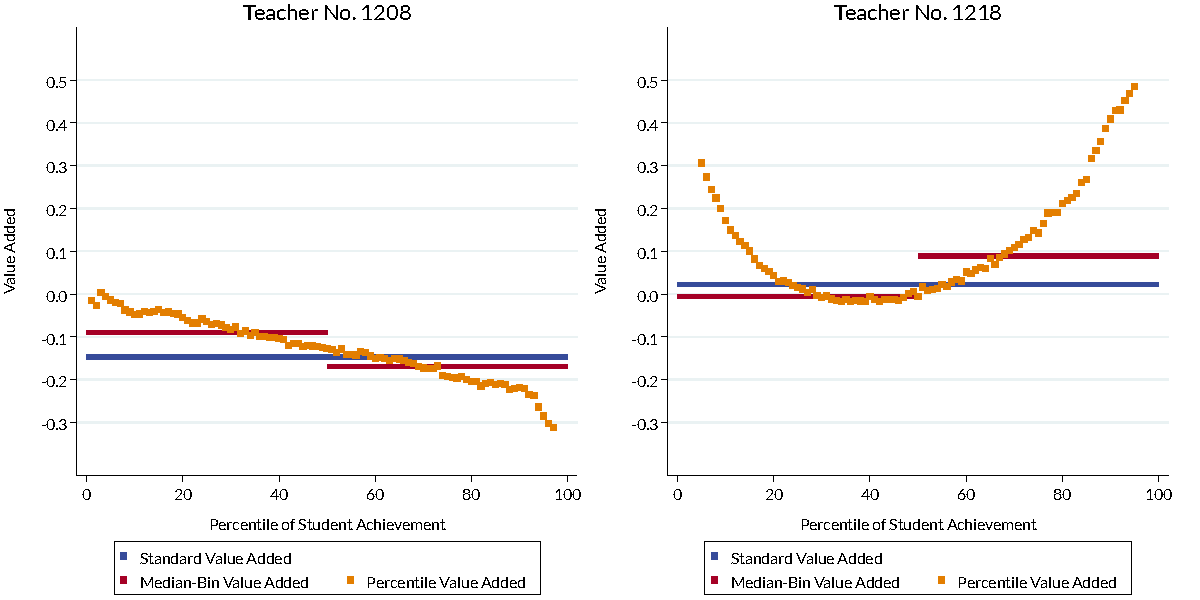
\includegraphics[width=.85\textwidth]{Working_Paper/WP_Figures/fig1_heterogeneity.pdf}
        \end{center}
            \caption{Teachers are Different}
               \label{fig_teacher_examples}
    \end{figure}

% needs to be updated! 
 \begin{figure}[H]
    \centering
    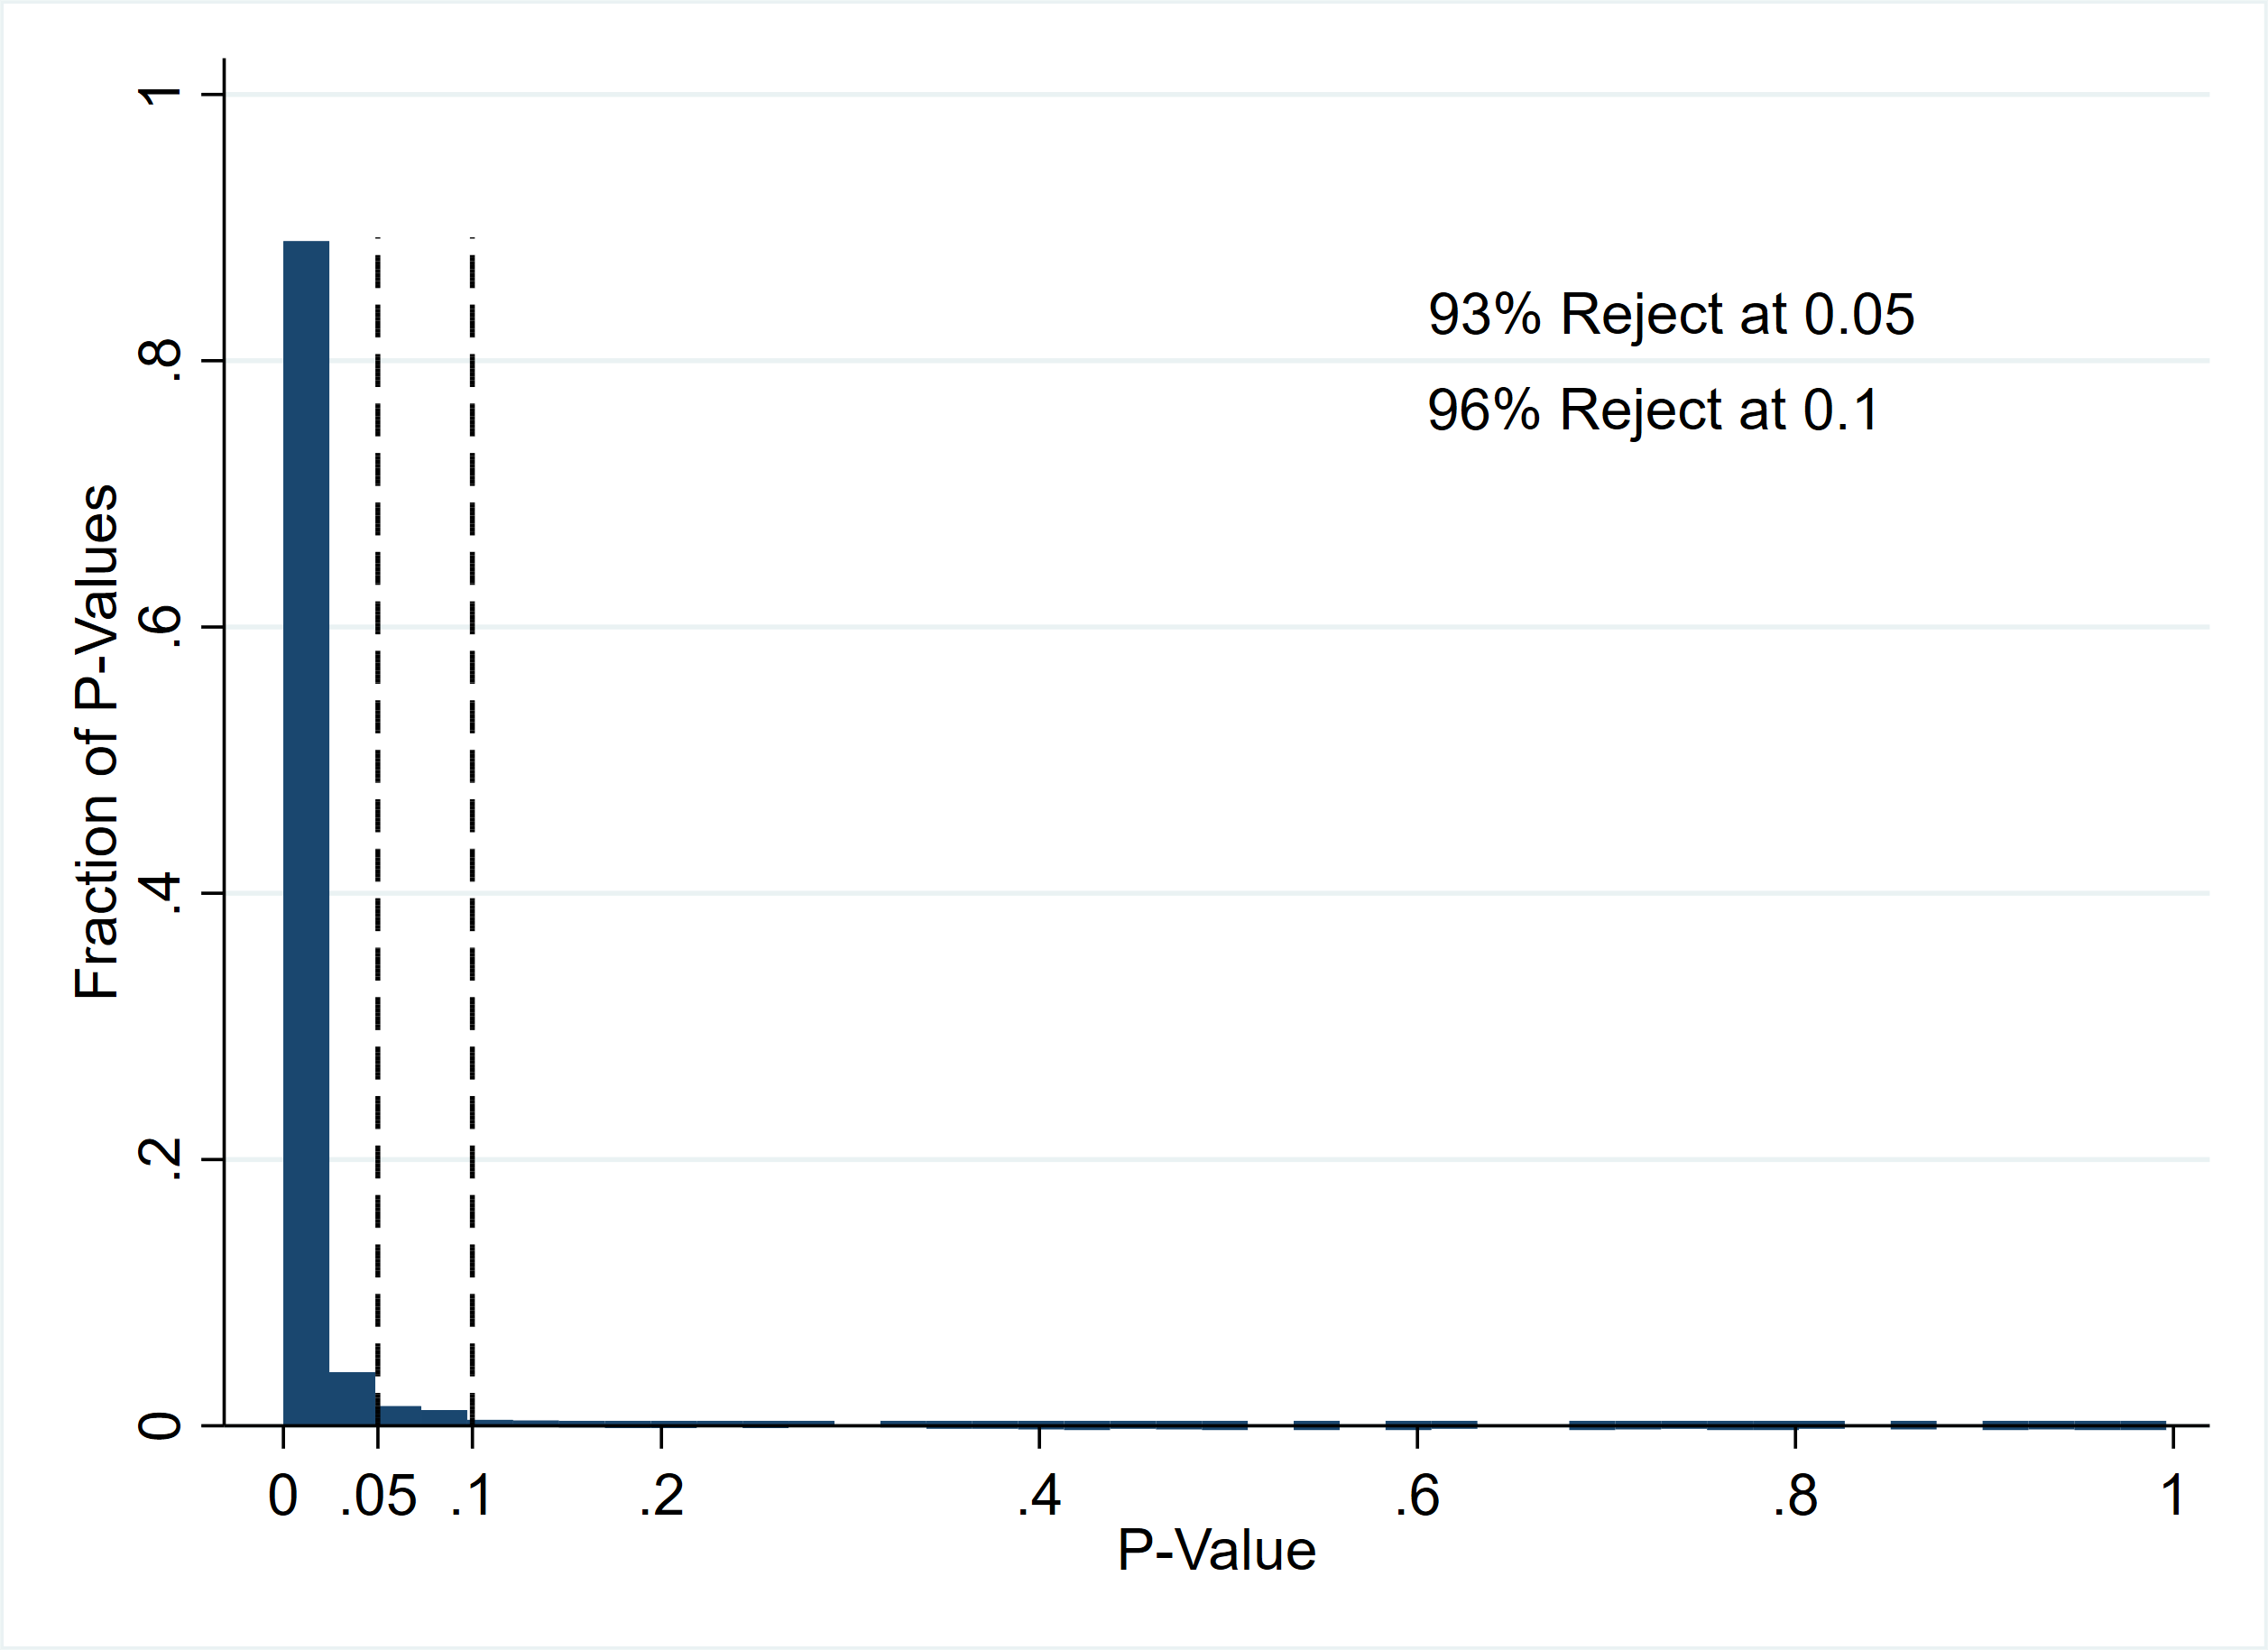
\includegraphics[width=.45\textwidth]{Working_Paper/WP_Figures/ELA_T_Test_Hist.png}
    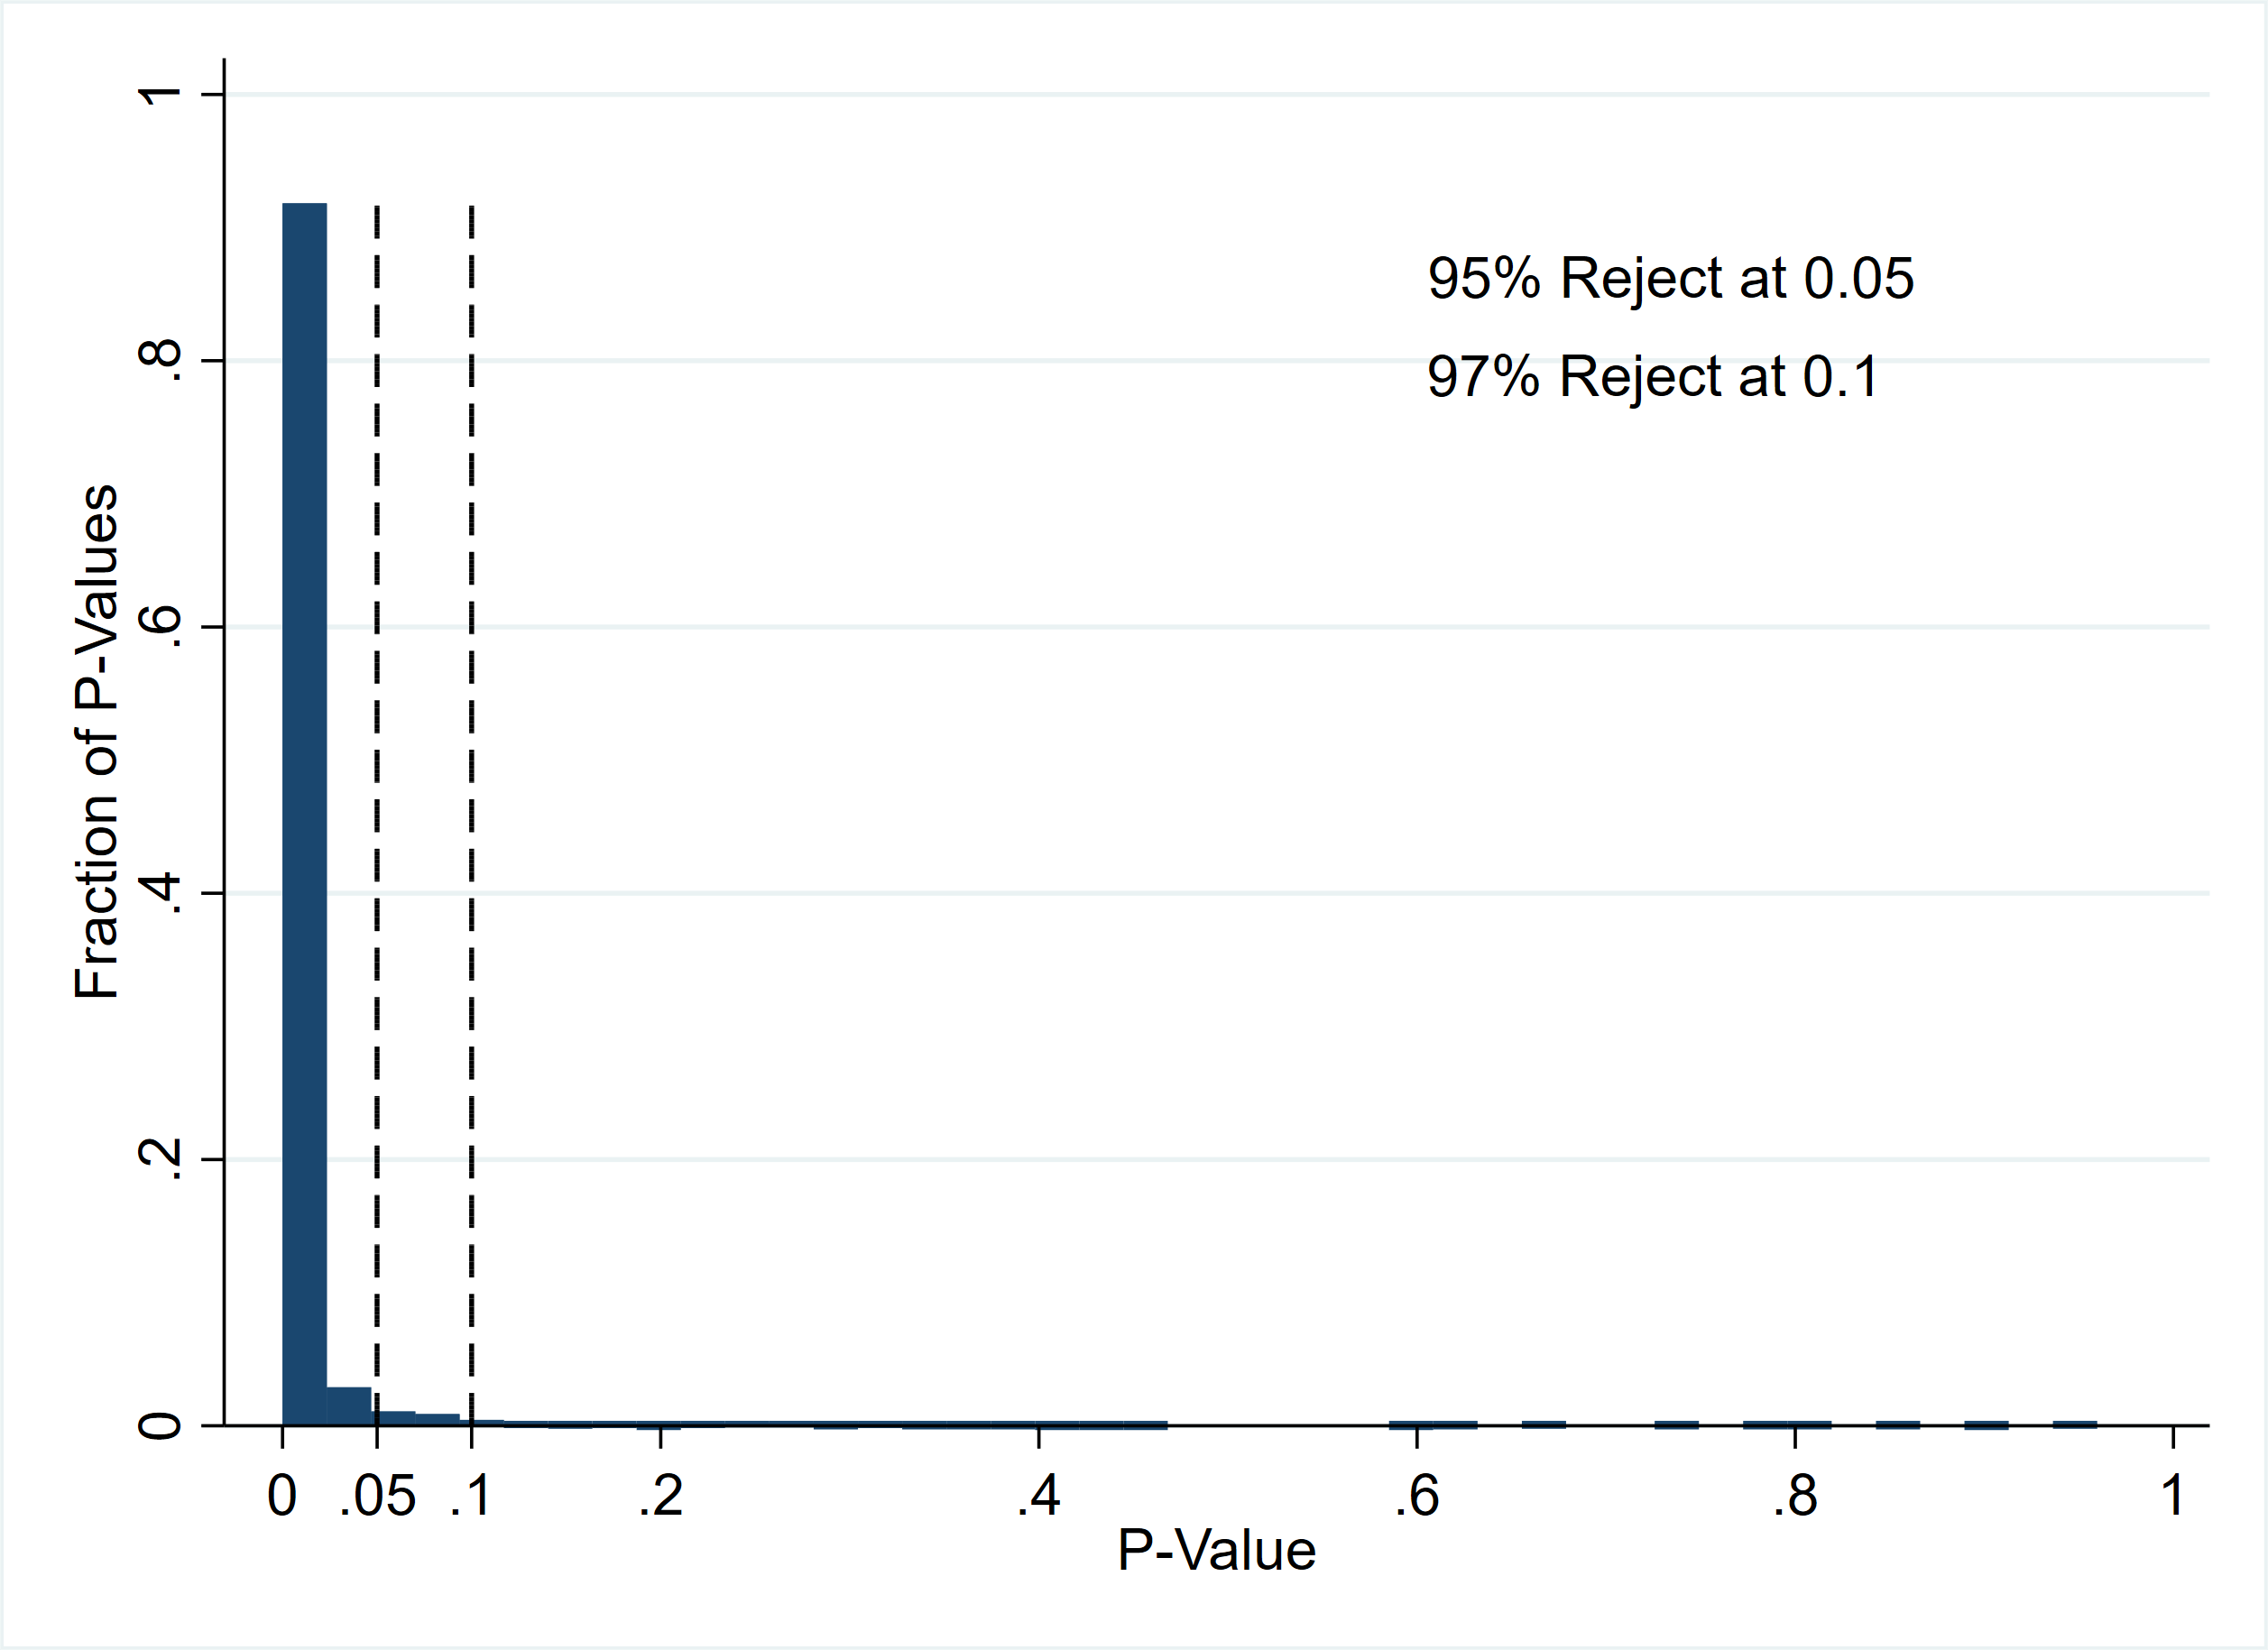
\includegraphics[width=.45\textwidth]{Working_Paper/WP_Figures/Math_T_Test_Hist.png}
      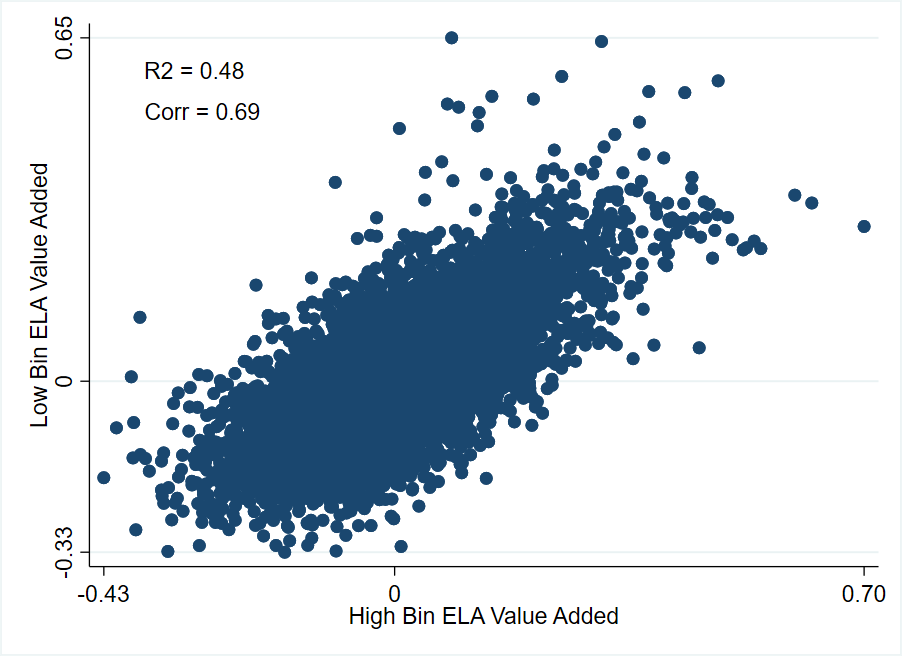
\includegraphics[width=.45\textwidth]{Working_Paper/WP_Figures/ELA_High_Bin_Versus_Low_Bin.png}
    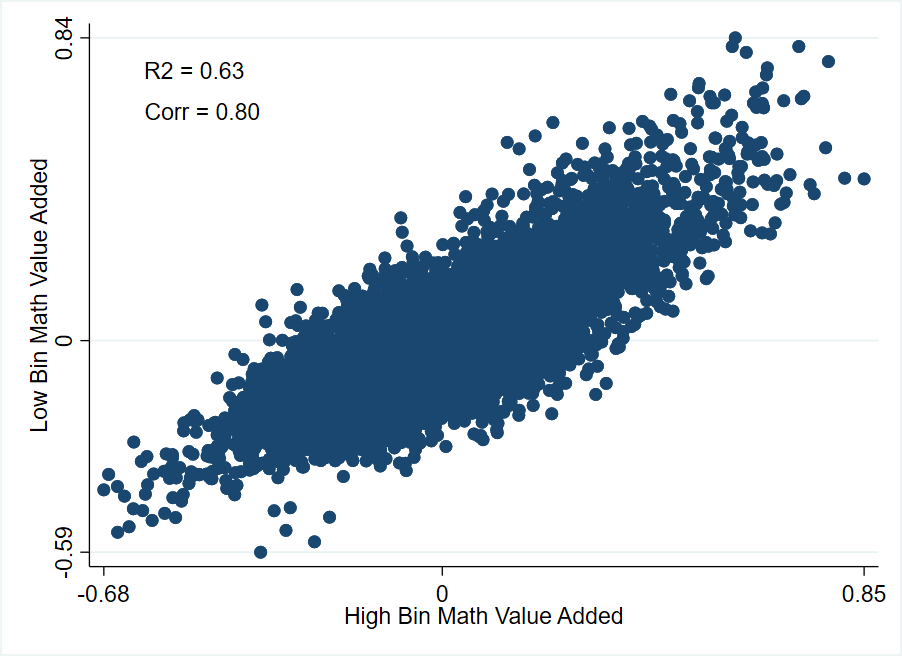
\includegraphics[width=.45\textwidth]{Working_Paper/WP_Figures/Math_High_Bin_Versus_Low_Bin.png}
        \caption{}
        \label{fig:t_tests}
\end{figure}

  
    
%%%%%%%%%%%%%%%%%%%%%%%%%%%%%%%%%%%%%%%
% Long-Term Impacts
%%%%%%%%%%%%%%%%%%%%%%%%%%%%%%%%%%%%%%%
\section{Long-Term Impacts} \label{long}

    The previous section makes it clear that heterogeneity does exist, and can be statistically detected. However, do the heterogeneous measures carry the same correlation with long term outcomes that standard value added does \citep{chetty2014measuring2}? In the spirit of \citet{chetty2014measuring2}, we validate these estimates in figure by exploring whether our results are predictive of various long term outcomes. Furthermore, we compare these associations with those provided by standard value added estimates in figure \ref{fig_long_term}. This helps us to better understand if we capture enough information with our flexible estimates compared to standard estimates.
    
    The outcomes we use are the following: `High School Grad' is an indicator for whether the student graduated from high school, `Two Year College' is an indicator for whether the student enrolled in a 2 year college within a year following high school graduation, `Four-Year College' is an indicator for whether the student enrolled in a 4 year college within a year following high school graduation, and `Any College' is an indicator for either `Two Year College' or `Four-Year College'. 
    
    Summary statistics for these outcomes are shown in figure \hl{TO DO}
    \begin{itemize}
        \item I want table or chart with the percent of students in each category. One possibility for the lack of an effect on HS gradation is high overall graduation rates which this will show. 
        \item I would also like to the see the distribution or average of test scores in grades 3-5 that reach each of these milestones. How many low score bin 5th graders are making it to college, for example. 
    \end{itemize}
    
    To test the predictive power of standard value added we run a regression of each of the outcomes described above on student demographics and the average teacher value added for the student in grades 3-5. For the binned estimates, rather than the average value added, we include terms for the average high bin value added of a student's teachers in grades 3-5 times an indicator for if that student is a high achieving student and a comparable term if they are a low bin student. This is analogous to treating the teacher bins as separate classrooms. The terms then indicate the predictive power of high bin value added on high scoring student's outcomes and low bin value added on low scoring student's outcomes. Figure \ref{fig_long_term} shows these coefficients for each of the outcome variables. 

    What does it look like for our heterogeneous measure to perform well? If our binned estimate corresponds to future outcomes in a similar way to standard value added, then the predictive power has not been diminished. Additionally, we might expect to see some additional information via idiosyncratic affects on particular outcomes. For example, we might expect the low bin value added to have a large affect on high-school graduation or two year-college while high bin has a larger impact on four year. 

    Our results for standard value added are somewhat consistent with what was found in \cite{chetty2014measuring2}. Surprisingly, none of the measures are predictive of high school graduation. I've been told the gradation rate is generally very high in SDUSC, which may be why value added has little affect, but will be able to say more once we get the summary statistics. While the standard errors keep most affects from being statically significant, standard value added and both of our binned estimates track closely with an increase in any college, primarily from four year college with potentially a drop in two year college, and an increase in a bachelor's degree within 6 years. While the standard errors are too large to say anything too confidently, the point estimates for two year college are higher for the low scoring bin, which makes sense if those students are closer to the margin of not going to any college. We can also see that the standard errors for each bin are not actually much bigger than for the mean as a whole. While a stronger difference in which outcomes are associated with which bins would give us an extra reason to focus on test score heterogeneity, the fact that they are closely matching the predicted outcomes of standard value added suggest we are not just picking up noise with the binned estimates. From this graph alone, it may not be clear why we would use the binned estimates at all though if it is conveying the same information. The following two sections connect the data to the theoy to give a clearer answer. 

    % updated 8/9/22
    \begin{figure}[H]
    \begin{center}
    \resizebox{!}{.02\textwidth}{
    $y_{i,j} = \sum_{k_j,k_i} \tau_{k_j,k_i} \hat{\gamma}_{j,k_j}\mathds{1}(k(i) = k_i) + \beta_2 X_i + \nu_{i,j}$}
    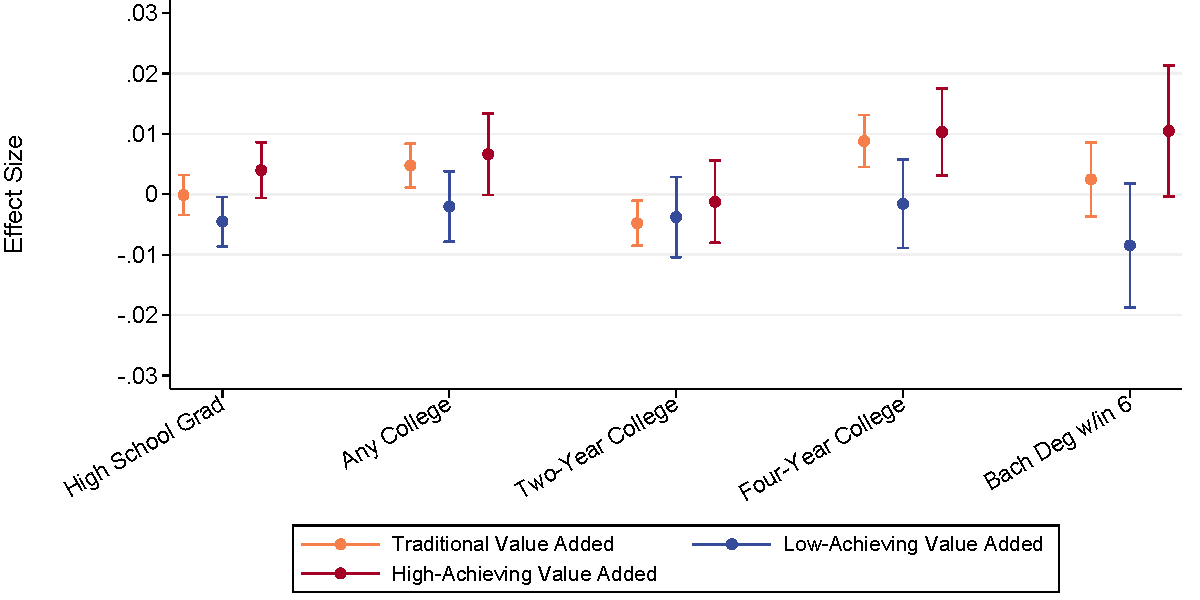
\includegraphics[width=.9\textwidth]{Working_Paper/WP_Figures/fig2b_longterm.pdf}
    \end{center}
        \caption{Long Term Effects}
        \label{fig_long_term}
    \end{figure}

%%%%%%%%%%%%%%%%%%%%%%%%%%%
% Implications for Students
%%%%%%%%%%%%%%%%%%%%%%%%%%%

\section{Implications for Students and Optimal Allocation of Teachers} \label{swell}

By estimating teacher value added flexibly along the student achievement distribution, policymakers can target gains in particular student sub-populations. To this end, we performed a set of teacher reallocation simulations using the estimated high and low bin value added for each teacher. In each simulation, we set a ‘weight’ $\alpha$ (between 0 and 1) on low bin students and $1 - \alpha$ on high bin students. In economic terms we are positing very simple linear indifference curves that trade off performance for below-median students with that of above-median students. A policymaker with these preferences may value gains to low score or high scoring students more, but does is not concerned with the distribution within each bin beyond the sum. The ‘weight’ on each group represents the degree to which policymakers wish to target gains between the two groups of students. We then rearranged teachers within school, grade, and year, keeping class composition fixed. We leave class composition fixed so that within-classroom peer effects are unchanged, and to avoid confounding changes in peer effects with changes in the teacher in each classroom. In particular, we found the welfare maximizing allocation based on each specified $\alpha$. We also include the average choices made by schools to compare against the welfare-maximizing outcomes. The results are shown in figure \ref{fig:aloc_eff}

% updated 8/9/22
\begin{figure}[H]
    \centering
    \resizebox{.3\textwidth}{!}{$\max_\mathcal{J} \mathcal{W}(\mathcal{J}) =  \sum_j \sum_{i\in j} \omega_{k(i)} \alpha_{j,{k(i)}}$}
    
    \begin{subfigure}[b]{0.45\textwidth}
    \subcaption[]{Within School ELA}
        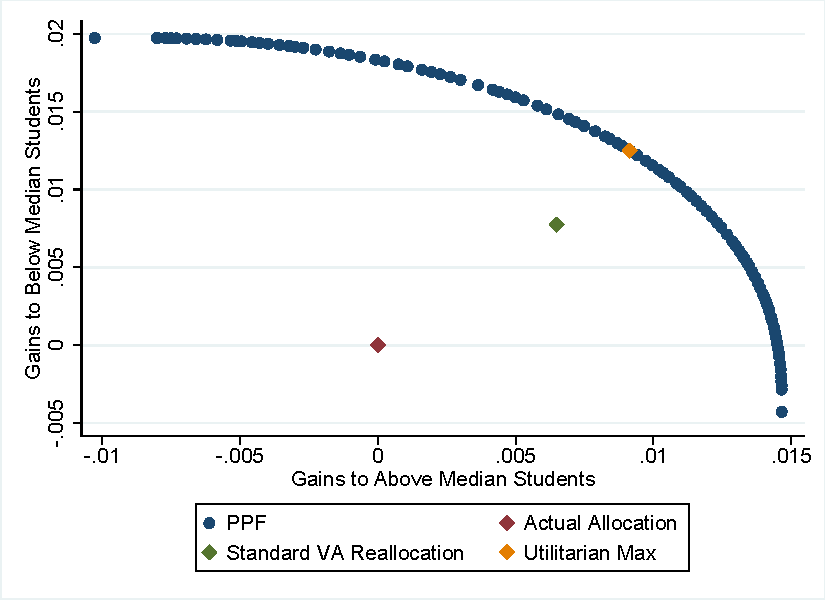
\includegraphics[width=1\textwidth]{Working_Paper/WP_Figures/WithinSchoolReallocationELA.pdf}
    \end{subfigure}
    \begin{subfigure}[b]{0.45\textwidth}
    \subcaption[]{Within School Math}
        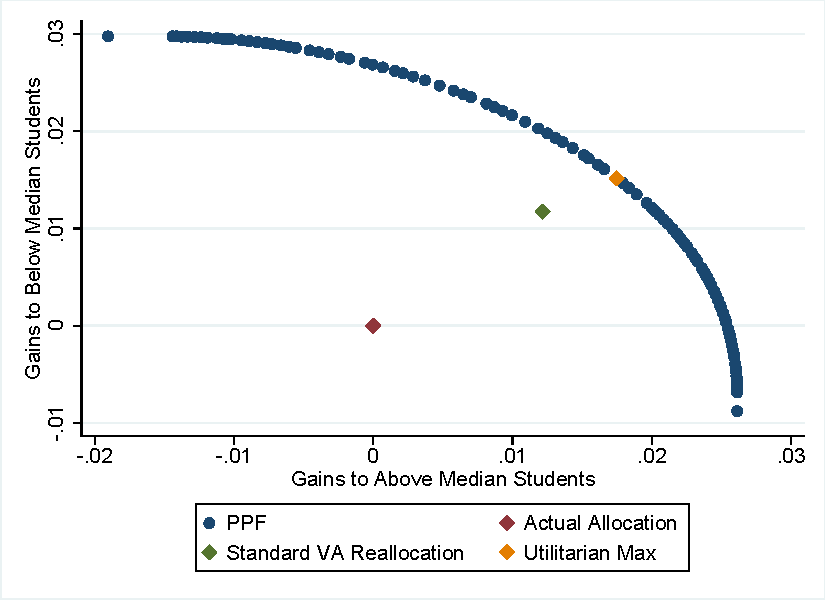
\includegraphics[width=1\textwidth]{Working_Paper/WP_Figures/WithinSchoolReallocationMath.pdf}
    \end{subfigure}
    \begin{subfigure}[b]{0.45\textwidth}
    \subcaption[]{Across School ELA}
        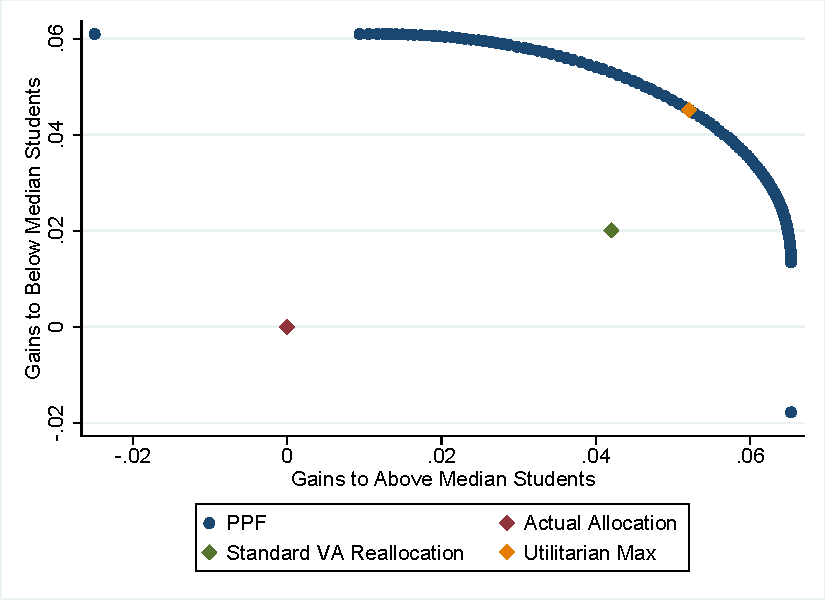
\includegraphics[width=1\textwidth]{Working_Paper/WP_Figures/AcrossSchoolReallocationELA.pdf}
    \end{subfigure}
    \begin{subfigure}[b]{0.45\textwidth}
    \subcaption[]{Across School Math}
        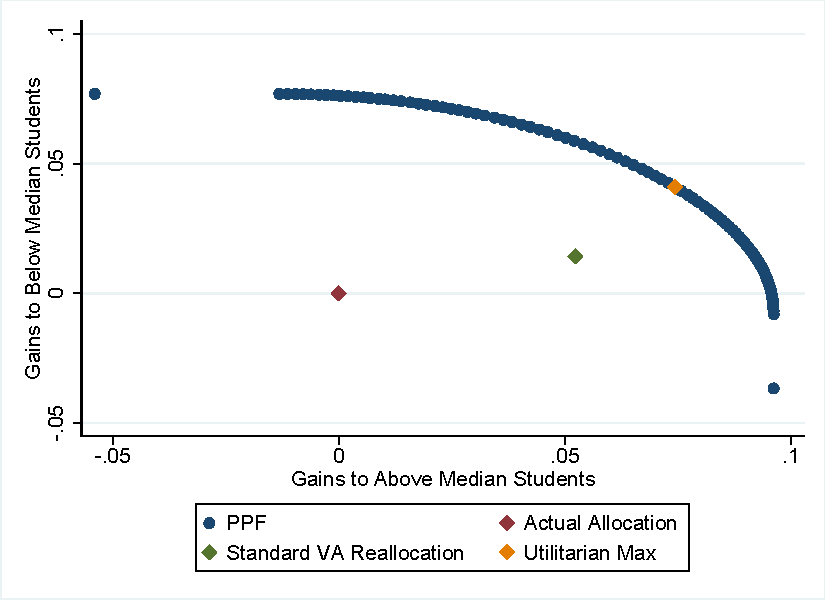
\includegraphics[width=1\textwidth]{Working_Paper/WP_Figures/AcrossSchoolReallocationMath.pdf}
    \end{subfigure}
    \caption{Allocative Efficiency}
    \label{fig:aloc_eff}
\end{figure}

	Each point in the figure represents the average gains to below median students (on the y-axis) and the average gains to above median students (on the x-axis) under the given reallocation. All gains have been re-centered on the actual allocation of teachers (the red diamond). This means, for example, if a point is at (-0.02, 0.04) that the simulation produced an average loss to above median students of 0.02 standard deviations and an average gain to below median students of 0.04 students, both relative to the actual allocation of teachers. The means a negative number indicates a ``loss" only relative to the future predicted by status quo policy and not that students are actually losing knowledge or getting lower test scores. 

	For reference, we marked the best reallocation with equal weight on all students $(\alpha=0.5)$ with an orange diamond. Additionally, we run a simulation where we order classes by size and teachers by standard value added within each school-grade-year cell, assigning the teacher with the highest standard value added to the biggest class, the next to the second biggest class, and so on until the teacher with the lowest standard value added gets the smallest class. This is represented on the figure by a green diamond.

	The first observation from these figures is that using the information gained with the two-bin estimates of value added allows for large possible gains on average for both above and below median students. Moving from the actual allocation to the utilitarian maximum within schools gives a rough average gain of 0.02 standard deviations to below median student and 0.015 to above median students in ELA (0.02 and 0.02 respectively in math). One thing to keep in mind with these gains is that they are estimates for a single year, so over time could compound for students who experienced these gains year on year. These gains also grow considerable if teachers are allocated across schools, .04 and .06 in ELA and .06 and .9 in math. 

	The second main takeaway from these figures is that there is a wide range of options for policymakers in deciding which students to target by deliberately assigning teachers to certain classes. Looking at the across school math allocations, for example, there is a .1 point swing in below median gains and a .15 swing in above median gains depending on the allocation chosen. This emphasizes the importance of thinking explicitly about welfare and the normative preferences of policymakers when making decisions like this. While standard value added may seam neutral, there is an implicit weight being used. 
 
	A final takeaway comes from considering the distance of the status quo – the red diamond – with the production possibility frontiers for maximizing welfare under the various weights. First, what does it mean for the actual allocation to be inside the frontier? Is it Pareto dominated? Not exactly. What we can say is that any policymaker with a welfare function that weights above and below median students with positive weights, but constant weights within each group, would prefer a point to the north east of the red dot. However, for other sets of welfare preferences, the red dot may be preferred. For example, a policymaker may favor a non-tested outcome or may care about some more nuanced subset of students, like the bottom or top decile of test scores. The potential concerns are limitless and so a true Pareto dominated outcome is unlikely to be found, but these figures show that, whatever choices are being made, they are coming at the expense of average above and below median gains.

    What gains or losses are being masked by these averages? After all, moving from the status quo to the egalitarian maximum involves moving teachers between classes. While there will be net gains from matching comparative advantages, some students will now be taught by less overall effective teachers or with a worse match for them despite the teacher being a better match for their class as a whole. The figures below give some idea of who is helped, harmed, or neither as we move along the frontier of allocations above (or, equivalently, reallocate teachers with a different ‘weight’ on below median students).
	
	In each figure (separated out for ELA and math scores/reallocations) the values on the y-axis are the gap between the simulated score and the actual realized score. Thus a .2 means that the student gains 0.2 standard deviations in the simulation and a -0.2 means a loss of -0.2 standard deviations in their test score relative to the realized score. Notably, in every simulation around one third of students keep the same teacher. This is reflected by a 0 on the y-axis and is the reason that the median in each box plot is at 0. Each box plot marks the 10th, 25th, 50th, 75th, and 90th percentiles over high and low bin students (marked by 1 and 0 respectively) and for several weights on low bin students (shown in the bottom row). Additionally, the mean in each category is marked with an “x”.

% updated 9/7/22
  \begin{figure}[H]
    \centering
     \begin{subfigure}[b]{0.45\textwidth}
    \subcaption[]{Within School ELA}
        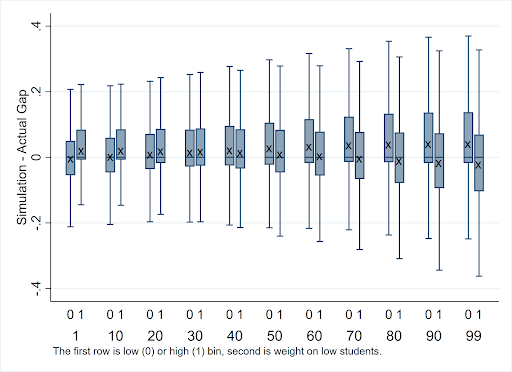
\includegraphics[width=1\textwidth]{Working_Paper/WP_Figures/ela_winners_losers.png}
    \end{subfigure}
     \begin{subfigure}[b]{0.45\textwidth}
    \subcaption[]{Within School Math}
        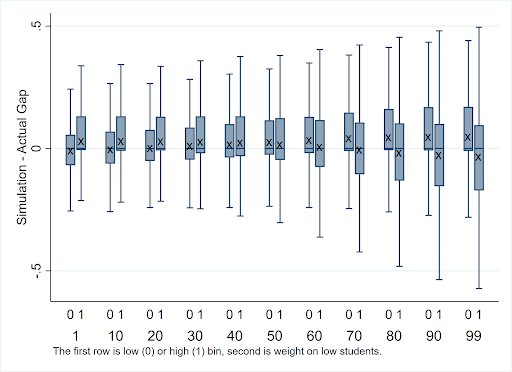
\includegraphics[width=1\textwidth]{Working_Paper/WP_Figures/Math_winners_losers.png}
    \end{subfigure}
    
    \label{fig:win_lose}
    \caption{Distribution of gains or losses for each bin across weighting schemes. \hl{Note these figure are not updated with newest chetty style estimation strategy}}
\end{figure}

Broadly these figures give us an idea that these policies must be thoughtfully implemented. 


Another important consideration for these simulations is what happens to achievement gaps as we move along the reallocation frontier? As expected, the one year reduction in average achievement gaps between above and below median student is quite high when reallocating students with more weight on low achieving students. In fact, the predicted reduction is roughly 0.1 sd in ELA and 0.12 sd in math.

	More interesting, though, is the reduction in achievement gaps for other student populations that we may care about. In fact, we can implement this completely race-blind policy (i.e. reallocating teachers to maximize welfare of above and below median students in terms of prior year achievement) and can reduce average racial test score gaps by 0.03 sd in ELA and 0.04 sd in math. 
 
% updated 9/7/22
 \begin{figure}[H]
    \centering
      \centering
     \begin{subfigure}[b]{0.45\textwidth}
    \subcaption[]{High and Low Test Score Gaps}
        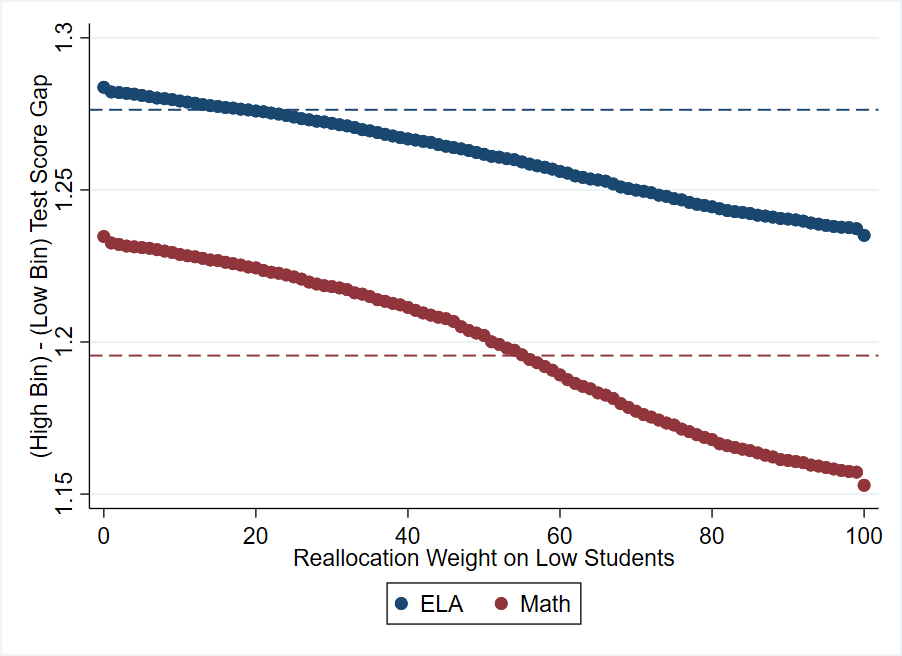
\includegraphics[width=1\textwidth]{Working_Paper/WP_Figures/test_score_gaps.png}
    \end{subfigure}
   \begin{subfigure}[b]{0.45\textwidth}
    \subcaption[]{Racial Gaps}
        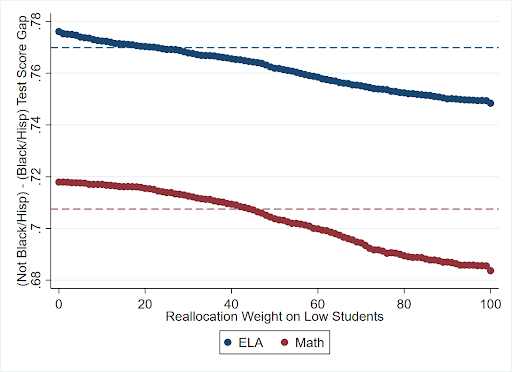
\includegraphics[width=1\textwidth]{Working_Paper/WP_Figures/race_gaps.png}
    \end{subfigure}
\end{figure}


%%%%%%%%%%%%%%%%%%%%%%%%%%%
% Implications for Teachers
%%%%%%%%%%%%%%%%%%%%%%%%%%%%%%%%%%
\section{Implications for Teachers} \label{twell}

The above example shows how measuring heterogeneity can improve student outcomes, but it can also be beneficial for teachers as well. A teacher Who has a class that does not fit their comparative advantage may not do well on standard value added assessments despite, perhaps, have similar skills to their peers. This issue is confounded by the third term in definition \ref{hetero_decomp}, which is the model mis-specification term. Suppose, for simplicity, value added is calculated with only a linear pretest control. If the actual relationship is S shaped, the line of best fit may, on average, have positive residuals for high scoring students and negative residuals for low scoring students. A teacher that has more low scoring students may mechanically get a lower value added score. We can see this in the differences between our aggregated heterogeneous estimates and the standard value added. For our aggregated estimates we weight the two bins equally, and yet we still find that standard value added disfavors black teachers relative to white teachers. \hl{this is also an older figure. I'm not certain how it will look with the newer estimation strategy, however, many district that use value added for incentive programs do not use the chetty approach and so this is also interesting in it's own right.}

% old, needs replacing 
\begin{figure}[H]
    \centering
    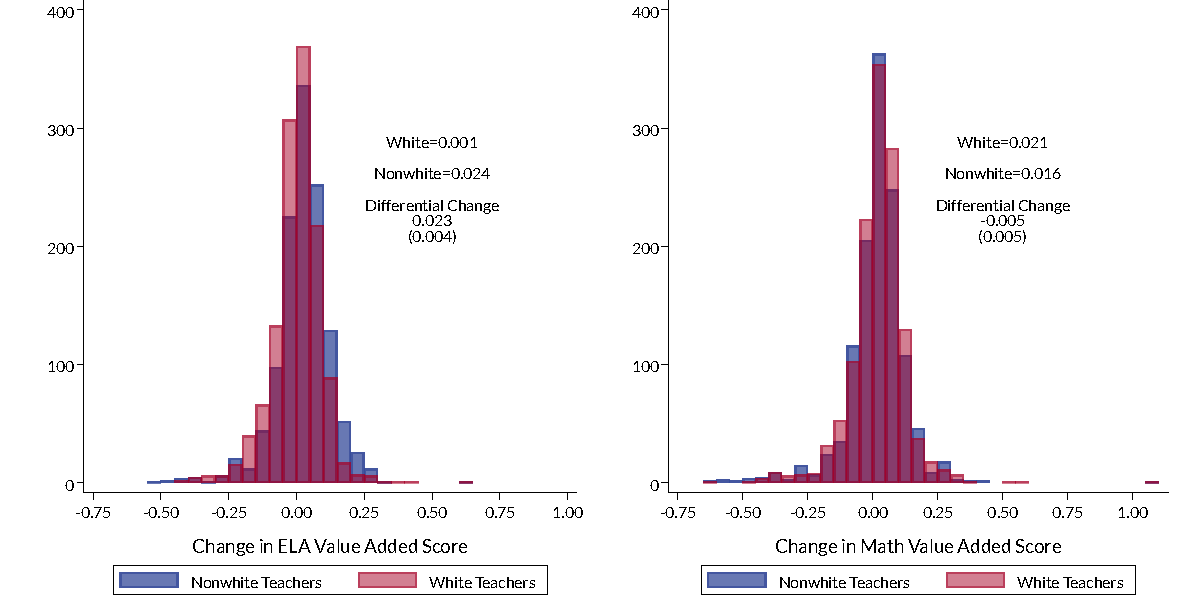
\includegraphics[width=.9\textwidth]{Working_Paper/WP_Figures/fig5_racial.pdf}
    \caption{Standard measures penalize minority teachers}
    \label{fig:my_label}
    
\end{figure}

We plan to plug these differences into a real payment scheme to see what the pay penalty for Black teacher's would be from standard value added compared to our aggregated heterogeneous measure. 

\section{Conclusion} \label{conc} 




\section{Appendix}

    %%%%%%%%%%%%%%%%%%%%%%%%%%%%%
    % Ordinal Test scores, Cardinal Welfare
   \subsection{Ordinal Test scores, Cardinal Welfare}
   \label{Cardinal_note}
    Some of the value of welfare weighting is that, with the proper welfare weights, we have transformed ordinal test scores to have actual cardinal meaning. The atonality of test scores has been shown to cause problems for Value Added inference \hl{(CITATION)}. Equal welfare weighted gains are meant to be equally valuable to the policymaker, so the welfare, sum of the weight and scores, have cardinal meaning that cannot be transformed even with an order preserving transformation. 
    
    Similar to welfare weights on utility, we are not requiring test scores (utility) to have ordinal meaning. We can transform test scores (utility), but will need a corresponding transformation of welfare weights to preserve the sum of the two (which is cardinal welfare). We can see this in the following numerical example. 
    
    Suppose you have a function of welfare weights for a set of linear scores $\gamma(S_i) = \frac{1}{s_i}$. So, a given change in scores from s1 to s2 gives a welfare change of $\int_{s_1}^{s_2} \frac{1}{s_i} = \ln(s_2)-\ln(s_1)$. This welfare has cardinal meaning, but test scores do not. So, we can transform the test scores with an order preserving transformation. For example let $t(s) = s^2$. to preserve our welfare measure, We just need a corresponding transformation of the welfare weights that gives a new function $\gamma_0(s)$ such that 
    $$\int_{t(s_1)}^{t(s_2)}\gamma_0(s)  = \ln(s_2)-\ln(s_1)$$
    
    $\gamma_0(s) = \frac{1}{2s}$ is such a transformation in this example. 
    
    In general if we let $\Gamma(s) = \int \gamma(s)$, then 
    
    $$ \frac{d \Gamma(t(s)) }{ ds} = \gamma_0(s) $$
    

\begin{table}[ht]
    \centering
    \renewcommand{\arraystretch}{1.2}

\begin{tabular}{lcccccc}
    \toprule
    \midrule
     & \multicolumn{3}{c}{ELA} & \multicolumn{3}{c}{Math} \\
     & Standard & Low & High & Standard & Low & High \\
    \midrule
    Masters & 0.010*** & 0.006** & 0.010*** & 0.020*** & 0.013*** & 0.021*** \\
     & (0.003) & (0.003) & (0.003) & (0.005) & (0.004) & (0.005) \\
    PhD & 0.012 & 0.021 & -0.021 & -0.011 & 0.006 & -0.010 \\
     & (0.024) & (0.021) & (0.021) & (0.036) & (0.031) & (0.036) \\
    Years Exp$^1$ & -0.009 & -0.004 & -0.033** & -0.144*** & -0.125*** & -0.150*** \\
     & (0.017) & (0.015) & (0.015) & (0.026) & (0.022) & (0.026) \\
    Black & 0.001 & 0.009 & 0.002 & -0.042*** & -0.015 & -0.052*** \\
     & (0.006) & (0.005) & (0.005) & (0.009) & (0.007) & (0.009) \\
    Asian & -0.011** & 0.001 & -0.024*** & -0.015 & 0.003 & -0.029*** \\
     & (0.006) & (0.005) & (0.005) & (0.008) & (0.007) & (0.008) \\
    Hispanic & 0.005 & 0.003*** & 0.001 & -0.002 & 0.004 & -0.002 \\
     & (0.004) & (0.003) & (0.003) & (0.006) & (0.005) & (0.006) \\
    Female & 0.011*** & 0.006** & 0.014*** & -0.002 & -0.000 & -0.003 \\
     & (0.003) & (0.003) & (0.003) & (0.005) & (0.004) & (0.005) \\
    \midrule
    $R^2$ & 0.004 & 0.003 & 0.009 & 0.008 & 0.005 & 0.011 \\
    N & 8,017 & 8,017 & 8,017 & 8,040 & 8,040 & 8,040 \\
    \midrule
    \bottomrule
\end{tabular}

    \label{tab:teacher_char}
    \bigskip
    
    \footnotesize{1 - Coefficients and standard errors in this row are multiplied by 100}
\end{table}








\pagebreak






\bibliography{citations}
\appendix
\captionsetup{labelformat=AppendixTables}


\setcounter{figure}{0}   
\setcounter{table}{0}   

\renewcommand{\thetable}{\arabic{table}}
\renewcommand{\thefigure}{\arabic{figure}}



\section{Data Appendix} \label{data_app}


\end{document}
